%% Elsevier elsarticle template for Computers & Operations Research

\documentclass[a4paper,fleqn]{cas-sc}

% Bibliography options - Harvard style for CAOR
% \biboptions{authoryear,longnamesfirst}
\usepackage[authoryear,longnamesfirst]{natbib}

% Your packages
\usepackage{amsmath,amssymb}
\usepackage{bm}
\usepackage{algorithm}    % defines the algorithm float
\usepackage{tabularx}
\usepackage{algpseudocode}  % defines \begin{algorithmic}, \State, ...
\usepackage{float}        % (optional) for [!t] placement specifier
\usepackage{booktabs}
\usepackage{pgfplots}
\usepackage{tikz}
\usetikzlibrary{matrix,calc}
\pgfplotsset{compat=1.18}

% , , , - Theorem-like environments , , , -
\usepackage{amsthm}
\newtheorem{theorem}{Theorem}
\newtheorem{lemma}[theorem]{Lemma}
\newtheorem{corollary}[theorem]{Corollary}
\theoremstyle{definition}
\newtheorem{definition}{Definition}
\newtheorem{remark}{Remark}
\newtheorem{assumption}{Assumption}
\newenvironment{pf}[1][Proof]{\begin{proof}[#1]}{\end{proof}}

\newcommand{\Occ}{\operatorname{Occ}}

\begin{document}
\let\WriteBookmarks\relax
\def\floatpagepagefraction{1}
\def\textpagefraction{.001}

% Main title
\title [mode = title]{The 2D Shortest Superstring Problem}
\shorttitle{The 2D Shortest Superstring Problem}


\author[vinuni]{Dat Thanh Tran\corref{cor1}}
\shortauthors{Dat Thanh Tran et al.}
\ead{dat.tt3@vinuni.edu.vn}
\author[vinuni]{Khai Quang Tran}
\ead{khai.tq@vinuni.edu.vn}
\author[vinuni]{Van Khu Vu}
\ead{khu.vv@vinuni.edu.vn}

\cortext[cor1]{Corresponding author}

\address[vinuni]{VinUniversity, Hanoi, Vietnam}

\begin{abstract}
The Shortest Superstring Problem (SSP), finding the shortest string containing a given set of strings as substrings, is a classical NP-hard problem. We introduce its two-dimensional generalization (2D-SSP): given a collection of rectangular symbol arrays, arrange them on the integer lattice with symbol-consistent overlaps to minimize bounding-box area. While 1D-SSP is pure sequencing, 2D-SSP becomes a \emph{simultaneous sequencing-and-packing} problem.

We prove NP-hardness for both the area and balanced-area objectives, and APX-hardness for the area objective via an L-reduction from 1D-SSP. We develop a \emph{Bounded-Offset Tree Representation} that transforms this geometric problem into a finite combinatorial problem over spanning trees. A connectivity lemma guarantees that optimal solutions can be made 4-connected without increasing cost, ensuring the tree space covers all optima.

Exploiting this representation, we design a Tree-Based Genetic Algorithm (T-GA) with \emph{locality-preserving crossover} that recombines subtrees rather than coordinates, preserving functional clusters across generations. Experiments verify near-optimality against exact ILP solvers (gap $\le 2.6\%$) and show 6--12\% improvement over greedy baselines on larger instances. The framework extends naturally to $d$ dimensions.
\end{abstract}

\begin{keywords}
Shortest superstring problem \sep Two-dimensional strings \sep Genetic algorithm \sep Integer linear programming \sep Combinatorial optimization \sep Bounded-offset tree encoding
\end{keywords}

\maketitle

% ===================== MAIN TEXT =====================

\section{Introduction}
\label{sec:intro}

The Shortest Superstring Problem (SSP) is a classical NP-hard problem~\citep{gallant1980finding}:
given a collection of strings, the goal is to construct the shortest string that
contains each input string as a contiguous substring. SSP has been extensively
studied, with known approximation algorithms~\citep{blum1994linear, mucha2013ssp} and rich connections to
combinatorial optimization.

This paper explores a largely uncharted territory at the intersection of two classical algorithmic domains: \emph{stringology} (the study of 1D sequencing problems like SSP, where overlap is the key operation) and \emph{bin packing} (the study of 2D geometric arrangement problems, where objects are placed without overlap). Standard packing algorithms fail when objects must overlap with symbol consistency; standard string algorithms fail when overlap can occur from four directions rather than two, and when a new object can fill an interior ``hole'' created by the arrangement of others. We introduce the \emph{Two-Dimensional Shortest Superstring Problem} (2D-SSP) as a principled bridge between these domains, providing both the theoretical foundations and algorithmic machinery to handle the unique challenges that arise when sequencing meets geometry.

In 2D-SSP, the basic objects are rectangular 2D strings $T_1,\dots,T_n$ (finite 2D arrays over a finite alphabet), collected into a set $\mathcal{T}$. The goal is to place them
in the plane with symbol-consistent overlaps so that all 2D strings are embedded while
minimizing a bounding-box cost derived from the minimal axis-aligned bounding rectangle enclosing the occupied region. We consider two cost variants:
\begin{itemize}
    \item the \emph{area objective}, which minimizes the rectangle area $H \cdot W$, the natural 2D generalization of string length in the classical SSP;
    \item a \emph{balanced-area objective}, which minimizes the side length $\max\{H,W\}$ of the smallest enclosing square, a secondary objective that penalizes extreme aspect ratios.
\end{itemize}

The primary motivation for 2D-SSP is \emph{compression}: just as 1D-SSP asks how compactly a set of strings can be represented via a single superstring exploiting overlaps, 2D-SSP asks the same question for 2D patterns. This is the natural higher-dimensional generalization of a classical problem, and to our knowledge, the first systematic study of SSP beyond one dimension. The problem exhibits a rich combinatorial structure---sitting at the intersection of stringology and geometric packing---that is absent from either domain alone and warrants study in its own right. Potential applications (DNA tile assembly, texture synthesis, 2D barcode design) may emerge where symbol-consistent overlap is physically meaningful, but our focus here is on establishing the theoretical and algorithmic foundations.

The transition from 1D to 2D introduces a fundamental \emph{complexity leap}. In 1D-SSP, strings can only overlap from two directions (left/right), making it a pure sequencing problem. In 2D-SSP, strings can overlap from four directions, and, crucially, a new string can fill a ``hole'' created by the arrangement of other strings. This transforms the problem into a \emph{simultaneous sequencing and packing} problem, where the optimal placement of one string depends not just on its neighbors but on the global geometric configuration. Our approach is the first to bridge these two domains by using a graph-based structure to handle the sequencing aspect and a grid-based canvas to handle the packing constraints.

Our central modelling innovation is a \emph{relative-offset encoding} that shifts the search space from absolute Cartesian coordinates to placement trees. Rather than representing a solution as an explicit 2D array or a vector of $(x,y)$ coordinates, we encode it as a \emph{tree of relative offsets between 2D strings}. This representation achieves \emph{symmetry-breaking} by collapsing the infinitely many translationally equivalent coordinate vectors into a single canonical form, and enforces structural connectivity by construction. Unlike coordinate-based representations, which suffer from high redundancy due to translational invariance, a solution at $(0,0)$ is equivalent to one at $(1,1)$, $(1,2)$, etc., our tree-based encoding ensures that each individual represents a \emph{unique relative arrangement}, significantly increasing search efficiency by eliminating redundant exploration of the coordinate space.

From a \emph{theoretical} perspective, we develop a \emph{Bounded-Offset Tree Representation} for 2D-SSP solutions. The key structural result (Theorem~\ref{thm:compaction}) shows that optimal placements can always be made 4-connected without increasing cost. This is intuitively similar to compaction arguments in VLSI floorplanning~\citep{murata1996vlsi}, but the proof is complicated by the \emph{symbol-consistency} constraint: we must verify that sliding disconnected components together does not introduce symbol conflicts, a concern absent in traditional floorplanning where components are non-overlapping rectangles. Building on this, we prove an \emph{Optimality-Preserving Equivalence} (Corollary~\ref{cor:tree-optimal}): every connected placement can be represented by a spanning tree of a naturally defined placement graph (though the correspondence is many-to-one: multiple trees may encode the same placement, and not every tree yields a feasible placement when decoded). Crucially, at least one optimal solution always admits such a tree representation, so the tree search space is \emph{complete} for optimization. Together, these results establish that \emph{the search space can be reduced from an infinite Cartesian plane to a finite discrete combinatorial space}, the space of spanning trees with bounded edge labels. While this space remains exponential in the worst case, it transforms a geometric optimization problem into a structured combinatorial one amenable to both exact methods and structure-aware search exploiting this bounded-offset encoding. Our theoretical framework (the connectivity/compaction theorem and tree representation) relies only on lattice adjacency and translation, making it directly applicable to $d$-dimensional generalizations for any $d \ge 2$.

From an \emph{algorithmic} perspective, the tree-based encoding enables a \emph{locality-preserving crossover} operator that directly addresses the \emph{building block hypothesis}~\citep{goldberg1989genetic}: a subtree corresponds to a spatially coherent cluster, and crossover can transplant entire subtrees between parents, preserving beneficial local arrangements. Our Tree-Based GA (T-GA) consistently outperforms greedy baselines and matches ILP-optimal solutions on small instances while scaling to much larger problems.

\section{Background and Related Work}
\label{sec:background}

\subsection{Shortest Superstring Problem}

In the classical SSP, the input is a set of strings
\[
\mathcal{S} = \{s_1,\dots,s_n\}
\]
over an alphabet \(\Sigma\). A superstring is a string \(S\) in which each
\(s_i\) appears as a substring. The objective is to minimize \(|S|\). SSP is
NP-hard, and there is a substantial literature on constant-factor
approximations (e.g., greedy maximum-overlap merging, cycle-cover-based
algorithms) and heuristic implementations used in practice.

\subsection{2D Covers and 2D Covering Sequences}

Two-dimensional generalizations of string concepts appear in several areas:
\begin{itemize}
    \item \emph{2D covers and 2D strings.} Work on covers of 2D arrays
    considers how a small pattern can cover a larger 2D string with overlaps,
    generalizing the notion of a cover in 1D~\citep{charalampopoulos2021covers}.
    \item \emph{Covering sequences and 2D covering sequences.} Recent research
    introduces covering sequences and covering 2D-sequences, where all
    $m \times n$ windows of a large 2D array form a covering code for patterns
    of that size up to a given radius. These provide natural sources of
    structured test instances~\citep{yehezkeally2025covering}.
\end{itemize}

These works focus on covering combinatorial spaces, whereas we focus on
overlapping a \emph{given finite set} of 2D strings with exact symbol consistency.

\subsection{2D Bin Packing and Cutting Stock}

Classical two-dimensional bin packing problems ask how to place a collection of
rectangles into one or more rectangular bins so as to minimize, for example,
the number of bins used or the height of a single strip, under strict
\emph{non-overlap} constraints. The items are unlabeled shapes. A closely related problem is the \emph{two-dimensional cutting stock problem}~\citep{gilmore1965multistage, lodi2002two}, where the goal is to cut rectangular pieces from large stock sheets while minimizing waste. Both problems have been extensively studied using exact methods (branch-and-bound, column generation) and metaheuristics (genetic algorithms, simulated annealing)~\citep{bennell2013tutorial}.

Our setting is similar in that we also optimize a global bounding box for a
family of rectangular pieces, but differs in two key ways. First, each string is
a \emph{discrete symbol array} rather than an unlabeled rectangle; second,
\emph{overlaps are allowed} as long as they are \emph{symbol-consistent}. Thus a
solution is not simply a packing of shapes, but a combinatorial ``gluing'' of
patterns in which overlaps can reduce the effective occupied area, a phenomenon
absent from standard 2D bin packing and cutting stock formulations. In the language of cutting stock, 2D-SSP allows ``pieces'' to share material when their patterns match, a constraint that transforms the problem from pure geometry to a hybrid of sequencing and packing.

\subsection{Related Geometric and Assembly Problems}

2D-SSP shares structural similarities with several problems in combinatorial optimization. In VLSI floorplanning, topological representations such as Sequence Pairs \citep{murata1995sequence} and B*-trees \citep{chang2000b} encode relative module positions; our placement trees adapt this approach to content-based adjacency. Patch-based texture synthesis \citep{efros2001image, kwatra2003graphcut} places patches to minimize visual error in overlaps; 2D-SSP is the discrete, lossless limit requiring exact symbol consistency. The Tile Assembly Model \citep{winfree1998algorithmic} studies self-assembly of Wang tiles with edge-matching constraints; 2D-SSP asks the inverse question of finding the most compact configuration containing a given set of patterned tiles. Unlike jigsaw puzzle assembly \citep{sholomon2013genetic} or polyomino packing \citep{golomb1994polyominoes}, 2D-SSP permits symbol-consistent overlaps that enable compression beyond pure geometric packing.

\section{Preliminaries}
\label{sec:problem}

In this section, we formalize the Two-Dimensional Shortest Superstring Problem (2D-SSP), introduce the two objective variants, and develop a \emph{Bounded-Offset Tree Representation} that enables structured algorithmic treatment. The central contribution of this section is showing that the search space can be reduced from an infinite coordinate space to a finite (though exponential) space of spanning trees with bounded edge labels. 

Let $\Sigma$ be a finite alphabet over which the 2D strings are defined. A \emph{2D-string} over $\Sigma$ is a finite
$m \times n$ array $T \in \Sigma^{m \times n}$, for some $m,n \in \mathbb{N}$.
For indices $1 \le i \le j \le m$ and $1 \le i' \le j' \le n$, we write
$T[i..j,\, i'..j']$ for the corresponding subarray and call this a
\emph{2D-substring} of $T$.

We identify a 2D string $T$ with a function on a finite index set
$C_T \subset \mathbb{Z}^2$, its set of \emph{local cell coordinates}.
We write cells as pairs $(u,v)\in\mathbb{Z}^2$ and use the same coordinate
system for both local and global positions: a translation by an offset
$p(i) = (x_i,y_i)$ sends a local cell $(u,v)$ of $T_i$ to the global cell
$p(i) + (u,v) = (x_i + u,\, y_i + v)$.
The choice of which axis is drawn horizontally or vertically is irrelevant
for our arguments; we only rely on coordinate-wise addition in $\mathbb{Z}^2$.

Let $P$ be an $m' \times n'$ 2D-string. We denote the set of its occurrences in
$T$ by
\[
\operatorname{Occ}(P,T) = \{(i,j) : T[i..i+m'-1,\; j..j+n'-1] = P\}.
\]

We will derive cost functions from the dimensions of the minimal axis-aligned
bounding rectangle of a placement, and consider two variants:
one that minimizes the area and one that minimizes the maximum side length (balanced-area objective).

\begin{definition}\label{def:2d-superstring}
Let $\mathcal{T} = \{T_1,\dots,T_n\}$ be a finite set of 2D strings over
$\Sigma$, which we call \emph{2D strings}. An $m \times n$ 2D-string $S$ is a
\emph{2D-superstring} of $\mathcal{T}$ if each string $T_i$ occurs as a
2D-substring of $S$, i.e.,
\[
    \operatorname{Occ}(T_i, S) \neq \emptyset
    \quad \text{for all } i \in \{1,\dots,n\}.
\]
We denote by
\[
    |S|_{\mathrm{area}} := m \cdot n
    \quad\text{and}\quad
    |S|_{\mathrm{bal}} := \max\{m,n\}
\]
the \emph{area} and the \emph{balanced side length} of $S$, respectively.
The area measure is the natural 2D analogue of string length in 1D-SSP, while the balanced measure constrains the aspect ratio.
Both are derived from the minimal axis-aligned rectangle containing $S$ and
penalize any empty cells inside that rectangle.
\end{definition}

Thus $|S|_{\mathrm{area}}$ is the primary objective, the natural 2D analogue of superstring length
(total cells in the bounding box), while $|S|_{\mathrm{bal}}$ is a constrained variant that bounds the aspect ratio,
ensuring neither dimension dominates.


\begin{figure}
\centering
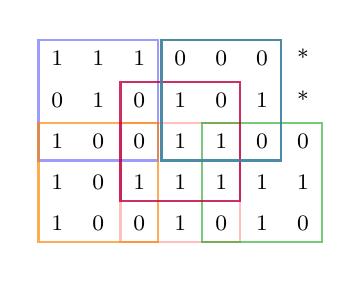
\begin{tikzpicture}[baseline=(m.center)]
\matrix (m) [matrix of nodes,
row sep=0pt, column sep=0pt,
nodes={minimum width=5.2mm, minimum height=5.2mm,inner sep=0pt, outer sep=0pt,font=\footnotesize}] {
1 & 1 & 1 & 0 & 0 & 0 & * \\
0 & 1 & 0 & 1 & 0 & 1 & *\\
1 & 0 & 0 & 1 & 1 & 0 & 0 \\
1 & 0 & 1 & 1 & 1 & 1 & 1 \\
1 & 0 & 0 & 1 & 0 & 1 & 0 \\
};
\draw[red,thick,opacity=0.250] ([xshift=0.6pt,yshift=-0.6pt]m-3-3.north west) rectangle ([xshift=-0.6pt,yshift=0.6pt]m-5-5.south east);
\draw[blue,thick,opacity=0.390] ([xshift=0.6pt,yshift=-0.6pt]m-1-1.north west) rectangle ([xshift=-0.6pt,yshift=0.6pt]m-3-3.south east);
\draw[green!60!black,thick,opacity=0.530] ([xshift=0.6pt,yshift=-0.6pt]m-3-5.north west) rectangle ([xshift=-0.6pt,yshift=0.6pt]m-5-7.south east);
\draw[orange,thick,opacity=0.670] ([xshift=0.6pt,yshift=-0.6pt]m-3-1.north west) rectangle ([xshift=-0.6pt,yshift=0.6pt]m-5-3.south east);
\draw[purple,thick,opacity=0.810] ([xshift=0.6pt,yshift=-0.6pt]m-2-3.north west) rectangle ([xshift=-0.6pt,yshift=0.6pt]m-4-5.south east);
\draw[cyan!60!black,thick,opacity=0.950] ([xshift=0.6pt,yshift=-0.6pt]m-1-4.north west) rectangle ([xshift=-0.6pt,yshift=0.6pt]m-3-6.south east);
\end{tikzpicture}
\caption{A 2D-superstring $S$ (5 rows $\times$ 7 columns) containing six 2D strings $T_1,\dots,T_6$ as 2D-substrings (highlighted rectangles). The cells marked with ``$*$'' are \emph{wildcard} (or \emph{don't-care}) positions, cells within the bounding box that are not covered by any input string. The area is $|S|_{\mathrm{area}} = 35$, and the balanced side length is $|S|_{\mathrm{bal}} = 7$.
}
\label{fig:cplex-seed342}
\end{figure}

\begin{remark}[Wildcard characters and 2D holes]
\label{rem:wildcard}
The wildcard symbol ``$*$'' in Figure~\ref{fig:cplex-seed342} represents a fundamental distinction between 1D-SSP and 2D-SSP. In 1D-SSP, every optimal superstring is \emph{fully covered}: each position belongs to at least one input string. If any position were uncovered, we could delete that character to obtain a shorter superstring, contradicting optimality.

In 2D-SSP, this property fails. The two-dimensional geometry permits \emph{holes}: cells within the bounding box that no input string covers. These holes cannot simply be ``deleted'' as in 1D, because removing a row or column would disrupt the geometric arrangement of strings in other parts of the superstring. The wildcard cells contribute to the bounding-box cost but carry no information, they can be filled with any symbol (or left undefined) without affecting which strings are embedded.

Formally, given a placement $p$, let $R(p) = \bigcup_{i=1}^n \mathrm{footprint}(T_i, p)$ denote the set of occupied cells, and let $B(p)$ denote the bounding box. The \emph{hole set} is $B(p) \setminus R(p)$, cells inside the bounding box but not covered by any string. In Figure~\ref{fig:cplex-seed342}, this set contains two cells (the ``$*$'' positions). These holes represent ``wasted'' area that inflates the objective value, and minimizing them is part of the optimization challenge unique to 2D-SSP.
\end{remark}

\begin{definition}
Given a finite set $\mathcal{T}$ of 2D strings over $\Sigma$, we define two
variants of the Two-Dimensional Shortest Superstring Problem:
\begin{itemize}
    \item \emph{Area-based 2D-SSP} (2D-SSP$_{\mathrm{area}}$): find a 2D-superstring $S$ of $\mathcal{T}$ minimizing $|S|_{\mathrm{area}}$. This is the primary variant, directly generalizing the 1D-SSP objective.
    \item \emph{Balanced-area 2D-SSP} (2D-SSP$_{\mathrm{bal}}$): find a 2D-superstring $S$ of $\mathcal{T}$ minimizing $|S|_{\mathrm{bal}}$. This variant constrains the aspect ratio and is useful in applications requiring near-square layouts.
\end{itemize}
Both objectives depend only on the minimal axis-aligned bounding rectangle of $S$ and penalize all empty cells inside it.
\end{definition}

\subsection{Computational complexity}

We establish that 2D-SSP is NP-hard. Both proofs are straightforward reductions; we state them for completeness.

\begin{theorem}[NP-hardness of 2D-SSP$_{\mathrm{area}}$]
\label{thm:np-hard}
2D-SSP$_{\mathrm{area}}$ is NP-hard, even for binary alphabets.
\end{theorem}

\begin{pf}
Reduction from 1D-SSP (NP-hard for $|\Sigma| \ge 2$~\citep{gallant1980finding}). Given 1D strings $\mathcal{S} = \{s_1, \ldots, s_n\}$, create height-1 2D strings $T_i = 1 \times |s_i|$. Any 2D placement with $k$ rows and maximum row width $W$ has area $\ge k \cdot W$. Concatenating rows yields a 1D superstring of length $\le k \cdot W$. Conversely, the optimal 1D superstring gives a 1-row 2D placement. Thus $\mathrm{OPT}_{2\text{D}} = \mathrm{OPT}_{1\text{D}}$.
\end{pf}

\begin{theorem}[NP-hardness of 2D-SSP$_{\mathrm{bal}}$]
\label{thm:np-hard-bal}
2D-SSP$_{\mathrm{bal}}$ is NP-hard.
\end{theorem}

\begin{pf}
Reduction from minimum enclosing square packing (NP-hard~\citep{leung1990packing}). Given rectangles $R_1, \ldots, R_n$, assign each a unique symbol $\sigma_i$ from alphabet $\Sigma$ with $|\Sigma| = n$. The resulting 2D strings cannot overlap (symbol conflict), so the problem reduces to non-overlapping rectangle packing.
\end{pf}

\begin{remark}[Complexity summary and open problems]
\label{rem:complexity-summary}
\emph{Area objective:} NP-hard and APX-hard for any $|\Sigma| \ge 2$ (inherited from 1D-SSP via L-reduction with $\alpha = \beta = 1$; see Appendix~\ref{app:apx-hardness}).

\emph{Balanced objective:} NP-hard, but Theorem~\ref{thm:np-hard-bal} requires a large alphabet ($|\Sigma| = n$). This places the proof in the \emph{packing regime} where no overlaps occur.

\textbf{Open problem:} \emph{The complexity of 2D-SSP$_{\mathrm{bal}}$ over a fixed constant-size alphabet (e.g., binary) remains open.} In the sequencing regime where overlaps are common, neither the 1D-SSP reduction nor the packing reduction applies directly.
\end{remark}

\subsubsection{Experimental scope}

Our experiments focus on the \emph{sequencing regime}: binary alphabets ($|\Sigma| = 2$) where overlap opportunities are common enough to matter but rare enough to be computationally challenging. This is the regime where 2D-SSP is most distinct from pure packing and where our tree-based methods provide the most value. See Appendix~\ref{app:complexity-details} for extended discussion of the sequencing--packing spectrum and entropy effects.

\medskip
Whenever the distinction between the two variants is not important, we simply refer to either as \emph{2D-SSP}. Hereafter, we use \emph{string} to mean \emph{2D string} unless otherwise specified.

We assume throughout that strings are axis-aligned rectangles and cannot be
rotated or reflected. Following standard 1D-SSP convention, we assume the input is \emph{substring-free}: no string $T_i$ is a 2D-substring of another string $T_j$. Redundant strings can be removed in polynomial-time preprocessing without affecting the optimal solution, since any 2D-superstring containing $T_j$ automatically contains $T_i$.

Rather than working directly with the superstring $S$, we use placements on the integer grid.

\begin{definition}
A \emph{placement} of $\mathcal{T}$ is a function
\[
    p : \{1,\dots,n\} \to \mathbb{Z}^2, \qquad p(i) = (x_i,y_i),
\]
assigning an integer offset to each string $T_i$. A cell of $T_i$ with local
coordinates $(u,v)$ (row and column indices) is mapped to global coordinates
$(x_i + u,\, y_i + v) \in \mathbb{Z}^2$.
\end{definition}

A placement $p$ is symbol-consistent if for every global coordinate $(x,y) \in \mathbb{Z}^2$, all strings covering $(x,y)$ under $p$ write the same symbol. We denote by
\[
\begin{aligned}
R(p) := \{(x,y) \in \mathbb{Z}^2 :\;
    & (x,y) \text{ is covered by some } T_i  \\
    & \text{under } p \}
\end{aligned}
\]
the union of occupied global cells, and let $B(p)$ be the minimal
axis-aligned rectangle containing $R(p)$. Let $W(p)$ and $H(p)$ be the width and height of $B(p)$, and define
\[
  \mathrm{cost}_{\mathrm{area}}(p) := W(p)\cdot H(p),
  \qquad
  \mathrm{cost}_{\mathrm{bal}}(p) := \max\{W(p),H(p)\}.
\]
Restricting the symbol map to $B(p)$ yields an $m \times n$ array $T_p$; by construction $T_p$ is a 2D-superstring of $\mathcal{T}$, and its area and balanced side satisfy
\[
|T_p|_{\mathrm{area}} = \mathrm{cost}_{\mathrm{area}}(p),
\qquad
|T_p|_{\mathrm{bal}} = \mathrm{cost}_{\mathrm{bal}}(p).
\]

In particular, empty cells of $B(p)$ that are not covered by any strings still contribute to both objectives.
Thus every symbol-consistent placement defines a feasible solution to both 2D-SSP$_{\mathrm{area}}$ and 2D-SSP$_{\mathrm{bal}}$, with cost equal to the chosen bounding-box functional.

\begin{remark}
\label{rem:bounding-box-justification}
We minimize bounding box area $W \cdot H$ rather than union area $|R(p)|$ for two reasons: (i) it is the natural 2D generalization of 1D superstring length, and (ii) minimizing $|R(p)|$ would permit fragmented layouts with ``holes,'' whereas bounding-box cost penalizes such fragmentation and encourages compact, connected arrangements.
\end{remark}

\begin{remark}
\label{rem:2d-vs-1d-optimality}
In 1D-SSP, every position in an optimal superstring must be covered by some input string. In 2D, the analogous condition, every row and column intersects some string, is necessary but not sufficient (Figure~\ref{fig:row-col-not-sufficient}). The connectivity/compaction theorem (Theorem~\ref{thm:compaction}) provides the appropriate 2D analogue by ensuring optimal placements can be made 4-connected.
\end{remark}

\begin{figure}
\centering
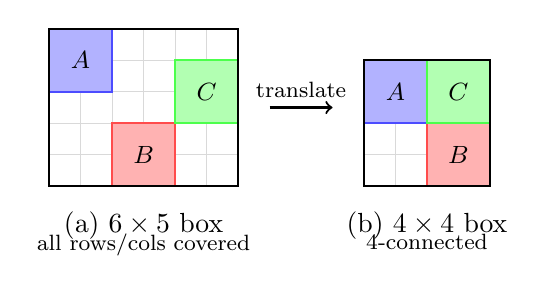
\begin{tikzpicture}[scale=0.4]
  % Grid for left placement (suboptimal)
  \draw[gray!30, very thin] (0,0) grid (6,5);
  
  % String A (top-left)
  \fill[blue!30] (0,3) rectangle (2,5);
  \draw[blue!70, thick] (0,3) rectangle (2,5);
  \node at (1,4) {\small $A$};
  
  % String B (bottom-right)  
  \fill[red!30] (2,0) rectangle (4,2);
  \draw[red!70, thick] (2,0) rectangle (4,2);
  \node at (3,1) {\small $B$};

  % String C (bottom-right)  
  \fill[green!30] (4,2) rectangle (6,4);
  \draw[green!70, thick] (4,2) rectangle (6,4);
  \node at (5,3) {\small $C$};
  
  \draw[thick] (0,0) rectangle (6,5);
  
  % Annotations
  \node[below] at (3,-0.5) {(a) $6 \times 5$ box};
  \node[below] at (3,-1.2) {\footnotesize all rows/cols covered};
  
  % Arrow
  \draw[->, thick] (7,2.5) -- (9,2.5);
  \node[above] at (8,2.5) {\footnotesize translate};
  
  % Grid for right placement (optimal)
  \begin{scope}[xshift=10cm]
    \draw[gray!30, very thin] (0,0) grid (4,4);
    
    % String A (top-left, same position)
    \fill[blue!30] (0,2) rectangle (2,4);
    \draw[blue!70, thick] (0,2) rectangle (2,4);
    \node at (1,3) {\small $A$};
    
    % String B (adjacent)
    \fill[red!30] (2,0) rectangle (4,2);
    \draw[red!70, thick] (2,0) rectangle (4,2);
    \node at (3,1) {\small $B$};

    % String C (adjacent)
    \fill[green!30] (2,2) rectangle (4,4);
    \draw[green!70, thick] (2,2) rectangle (4,4);
    \node at (3,3) {\small $C$};

    \draw[thick] (0,0) rectangle (4,4);
    
    \node[below] at (2,-0.5) {(b) $4 \times 4$ box};
    \node[below] at (2,-1.2) {\footnotesize 4-connected};
  \end{scope}
\end{tikzpicture}
\caption{Row/column coverage is necessary but not sufficient for 2D optimality. (a)~Both strings cover all rows and columns of the $6 \times 5$ bounding box, yet they are disconnected. (b)~Translating $B$ diagonally yields a 4-connected placement with a smaller $4 \times 4$ bounding box.}
\label{fig:row-col-not-sufficient}
\end{figure}

Conversely, let $S$ be a 2D-superstring of $\mathcal{T}$ and fix
an arbitrary occurrence $(i,j) \in \operatorname{Occ}(T_k,S)$ for each string $T_k$.
Placing $T_k$ with offset $(i,j)$ then yields a symbol-consistent
placement whose induced array is $S$ up to a global translation.
Hence optimizing over 2D-superstrings is equivalent to optimizing
over symbol-consistent placements, modulo a global shift of all
coordinates.  We therefore work with placements from now on.

A subset $R \subseteq \mathbb{Z}^2$ is \emph{4-connected} if its adjacency graph
under the 4-neighbourhood ($\|x-y\|_1 = 1$) is connected. Two cells
$x,y\in\mathbb{Z}^2$ overlap if $x=y$.

\begin{definition}
\label{def:placement-graph}
Given the string set $\mathcal{T}$, the \emph{placement graph} $G^{\mathrm{pl}}$
has vertex set $\{1,\dots,n\}$. Its edges are triples
\[
    e = (i,j,\delta) \quad\text{with}\quad i \neq j,\; \delta \in \mathbb{Z}^2,
\]
where $\delta$ is a relative offset such that placing $T_j$ at position
$p(j) = p(i) + \delta$ yields symbol-consistent contact between $T_i$ and $T_j$, meaning they either overlap with matching symbols, or are 4-adjacent (share a boundary edge). Multiple edges may exist for the same unordered pair $\{i,j\}$, corresponding to different valid offsets.
\end{definition}

Intuitively, each edge $(i,j,\delta)$ in $G^{\mathrm{pl}}$ specifies a way of
gluing $T_j$ next to $T_i$. The placement graph is determined entirely by $\mathcal{T}$ and can be precomputed before searching for solutions.

\begin{lemma}
\label{lem:bounded-offsets}
Let $T_i$ and $T_j$ have bounding boxes of dimensions $w_i \times h_i$ and $w_j \times h_j$. If $(i,j,\delta)$ is an edge in $G^{\mathrm{pl}}$, then $\delta = (\Delta x, \Delta y)$ satisfies:
\[
|\Delta x| \le w_i + w_j - 1, \qquad |\Delta y| \le h_i + h_j - 1.
\]
\end{lemma}

\begin{pf}
For $T_i$ and $T_j$ to be in contact (overlap or 4-adjacent), their bounding boxes must intersect or share an edge. The $x$-projections $[0, w_i-1]$ and $[\Delta x, \Delta x + w_j - 1]$ intersect or are adjacent if $|\Delta x| \le w_i + w_j - 1$. The bound for $\Delta y$ follows symmetrically.
\end{pf}

\begin{remark}[Graph size vs.\ tree space]
\label{rem:polynomial-search}
Lemma~\ref{lem:bounded-offsets} ensures that the \emph{placement graph} $G^{\mathrm{pl}}$ has polynomial size: for each pair $(T_i, T_j)$, there are $O((w_i + w_j)(h_i + h_j))$ candidate offsets to check. For uniform $w \times h$ strings, the placement graph has $O(n^2 wh)$ edges.

However, the \emph{search space of spanning trees} remains exponential. By Cayley's formula, a complete graph on $n$ vertices has $n^{n-2}$ spanning trees; while our placement graph is typically sparser, the number of feasible placement trees can still grow exponentially with $n$. The significance of our reduction is not that it yields a polynomial search space, but that it transforms an \emph{infinite continuous space} (absolute coordinates on $\mathbb{Z}^2$) into a \emph{finite discrete combinatorial space} (spanning trees with bounded edge labels). This discretization enables exact enumeration for small instances and structured search exploiting the graph-based encoding for larger ones.
\end{remark}

\begin{remark}[Edge density]
\label{rem:edge-density}
The bound $O(n^2 wh)$ on $|E(G^{\mathrm{pl}})|$ is a worst-case geometric bound. The actual edge count depends on string entropy: high-entropy strings yield sparse graphs (dominated by adjacency edges), while low-entropy strings yield dense graphs (many symbol-consistent overlaps). See Appendix~\ref{app:edge-density} for detailed analysis.
\end{remark}

\begin{remark}[Optimized offset enumeration]
\label{rem:offset-enumeration}
In the sequencing regime, practical performance improves by enumerating offsets in order of bounding-box increase, stopping at the first level with a symbol-consistent offset. See Appendix~\ref{app:offset-enumeration} for details.
\end{remark}

\begin{definition}
\label{def:contact-graph}
Let $p$ be a symbol-consistent placement of $\mathcal{T}$. The
\emph{contact graph} $G^{\mathrm{ct}}(p)$ is the subgraph of $G^{\mathrm{pl}}$ induced by $p$: it has vertex set $\{1,\dots,n\}$, and edge $(i,j,\delta)$ is present if $\delta = p(j) - p(i)$ and this edge exists in $G^{\mathrm{pl}}$.

Equivalently, strings $i$ and $j$ are adjacent in $G^{\mathrm{ct}}(p)$ if they are in contact under $p$ (overlapping or 4-adjacent).
\end{definition}

The contact graph $G^{\mathrm{ct}}(p)$ records which edges of the placement graph are ``realized'' by a given placement. Different placements of the same instance may realize different subsets of edges.

\begin{remark}
Our cost functionals depend only on the bounding rectangle $B(p)$, not directly on the cardinality of $R(p)$. In particular, two placements with the same bounding box have the same cost for both 2D-SSP$_{\mathrm{area}}$ and 2D-SSP$_{\mathrm{bal}}$. The area-based objective directly generalizes the 1D shortest superstring objective (string length), while the balanced-area variant additionally constrains the aspect ratio. Both differ from geometric covering formulations that minimize the area of the union $R(p)$.
\end{remark}

\begin{assumption}
\label{ass:connected-union}
In the structural discussion below we work with placements
whose occupied region $R(p)$
is 4-connected. The following theorem shows this is without loss of optimality.
\end{assumption}

The following theorem shows that optimal solutions can be restricted to connected placements, a result analogous to compaction in VLSI floorplanning~\citep{murata1996vlsi}.

\begin{theorem}[Connectivity/compaction]
\label{thm:compaction}
Let $p$ be an optimal symbol-consistent placement for 2D-SSP (under either $\mathrm{cost}_{\mathrm{area}}$ or $\mathrm{cost}_{\mathrm{bal}}$). If $R(p)$ is not 4-connected, then there exists an optimal symbol-consistent placement $p'$ such that $R(p')$ is 4-connected and $\mathrm{cost}(p') \le \mathrm{cost}(p)$.
\end{theorem}

\begin{pf}
We prove existence of an optimal 4-connected placement by an extremal argument.

\medskip
\noindent\textbf{Canonical normalization and tie-breaking.}
Among all optimal symbol-consistent placements (for the chosen objective), pick one $q$ as follows.
First translate $q$ so that the lower-left corner of its bounding box is at the origin, i.e., $B(q)=[0, W-1]\times[0, H-1]$ for some $W,H$.
Among all such translated optimal placements, choose $q$ that minimizes the pair $(W,H)$ lexicographically, and subject to that minimizes
\[
  \Phi(q) := \sum_{(x,y)\in R(q)} x \; + \; \sum_{(x,y)\in R(q)} y.
\]
This tie-breaking is well-defined because, after anchoring $B(q)$ at the origin, the set $R(q)\subseteq [0,W-1]\times[0,H-1]$ is finite.

\medskip
\noindent\textbf{Claim: $R(q)$ is 4-connected.}
Assume for contradiction that $R(q)$ has at least two maximal 4-connected components.
Let these components be $C_1,\dots,C_k$ with $k\ge 2$.

\smallskip
\noindent\emph{(1) Components are separated by distance at least 2.}
For distinct components $C_i\neq C_j$, we have $\mathrm{dist}(C_i,C_j)\ge 2$: if $\mathrm{dist}(C_i,C_j)=1$ then there exist 4-adjacent cells across them, contradicting maximality of 4-connected components.

\smallskip
\noindent\emph{(2) Any unit shift of a component cannot create overlap.}
Fix a component $C$ and a unit vector $e\in\{(\pm1,0),(0,\pm1)\}$.
If $(C+e)\cap (R(q)\setminus C)\neq\emptyset$, then there exist $c\in C$ and $d\in R(q)\setminus C$ with $c+e=d$, hence $\|c-d\|_1=1$ and thus $\mathrm{dist}(C, R(q)\setminus C)=1$, contradicting (1).
Therefore shifting any component by a unit step preserves non-overlap with all other components.
Since the shift is rigid, symbol-consistency is preserved as well.

\smallskip
\noindent\emph{(3) Each component touches every side of the bounding box.}
Suppose some component $C$ does not touch the left side of $B(q)$, i.e., every cell $(x,y)\in C$ satisfies $x\ge 1$.
Then $C+(-1,0)\subseteq B(q)$.
By (2), translating $C$ by $(-1,0)$ yields a symbol-consistent placement $q'$ whose occupied set stays inside the same box $B(q)$, so $(W,H)$ does not increase.
However, this translation strictly decreases $\Phi$ (every cell of $C$ decreases its $x$-coordinate by 1), contradicting the choice of $q$.
Thus every component touches the left side.
The same argument applied to $(1,0)$, $(0,-1)$, and $(0,1)$ shows that every component touches the right, bottom, and top sides of $B(q)$.

\smallskip
\noindent\emph{(4) Two disjoint components cannot both touch all four sides.}
Fix two distinct components $A$ and $B$.
Since $A$ is 4-connected and touches the left and right sides, it contains a 4-neighbour path in the grid from the left side of $B(q)$ to the right side.
Similarly, since $B$ is 4-connected and touches the top and bottom sides, it contains a 4-neighbour path from the top side to the bottom side.
By the standard planar separation (crossing) property of the rectangular grid (see Lemma~\ref{lem:grid-crossing} in Appendix~\ref{app:grid-crossing}), these two paths must share a grid cell.
This contradicts that $A$ and $B$ are disjoint.

Therefore $k=1$ and $R(q)$ is 4-connected.

\medskip
\noindent\textbf{Conclusion.}
Let $p':=q$. Then $p'$ is optimal for the chosen objective and $R(p')$ is 4-connected.
In particular, $\mathrm{cost}(p')=\mathrm{cost}(q)\le \mathrm{cost}(p)$.
\end{pf}

\begin{corollary}
For any instance of 2D-SSP, there exists an optimal placement whose occupied region is 4-connected. Consequently, Assumption~\ref{ass:connected-union} is justified for all instances.
\end{corollary}

This connectivity/compaction theorem establishes that restricting attention to connected placements loses no optimal solutions. The assumption matches our experimental
focus and enables the tree-based structural perspective developed in this section. It is not required for the correctness of the algorithms in
Section~\ref{sec:algorithms}, which operate on arbitrary
symbol-consistent placements.

\begin{corollary}[Connected occupied region implies connected contact graph]
\label{cor:contact-connected}
Let $p$ be a symbol-consistent placement such that $R(p)$ is 4-connected.
Then the contact graph $G^{\mathrm{ct}}(p)$ is connected.
\end{corollary}

\begin{pf}
If $G^{\mathrm{ct}}(p)$ were disconnected, we could partition the strings into
two nonempty sets $A$ and $B$ with no edge between them. For each string $T_i$, let $R_i$ be the set of global cells covered by $T_i$
under $p$. Define
\[
  R_A = \bigcup_{i\in A} R_i,
  \qquad
  R_B = \bigcup_{j\in B} R_j,
\]
so that $R(p) = R_A \cup R_B$ and $R_A \cap R_B = \emptyset$.
By construction there is no pair of 4-adjacent cells across $R_A$ and $R_B$,
which contradicts 4-connectivity of $R(p)$.
\end{pf}

By Theorem~\ref{thm:compaction} and Corollary~\ref{cor:contact-connected},
every optimal connected placement has a connected contact graph that admits a spanning tree. We now formalize this tree representation.

\subsection{Placement trees}

A placement tree encodes a solution as a spanning tree with labeled edges specifying relative offsets between strings. The key insight is that edge labels are drawn from a \emph{bounded} set determined by string dimensions, which, combined with the finite number of spanning tree topologies, yields a finite search space.

\begin{definition}\label{def:placement-tree}
A \emph{placement tree} for $\mathcal{T}$ is a rooted tree
$F = (V,E)$ with vertex set $V = \{1,\dots,n\}$ together with, for each
edge $\{i,j\} \in E$, a label $\delta_{ij} \in \mathbb{Z}^2$ interpreted as
the relative offset from $i$ to $j$.
For each oriented edge $(i,j)$ we store $\delta_{ij}$ and require
$\delta_{ji} = -\delta_{ij}$.

By Lemma~\ref{lem:bounded-offsets}, valid edge labels are bounded: if $T_i$ and $T_j$ have dimensions $w_i \times h_i$ and $w_j \times h_j$, then any symbol-consistent contact requires $|\Delta x| \le w_i + w_j - 1$ and $|\Delta y| \le h_i + h_j - 1$. This bounds the number of candidate labels per edge to $O((w_i + w_j)(h_i + h_j))$---for uniform $w \times h$ strings, $O(wh)$ per edge---ensuring the search space of placement trees is finite.

The \emph{realization} of $F$ with root $r$ and root position
$p(r)\in\mathbb{Z}^2$ is the placement $p_F$ defined by
\[
  p_F(i)
  \;=\;
  p(r) + \sum_{t=0}^{\ell-1} \delta_{v_t v_{t+1}},
\]
where $r = v_0, v_1, \dots, v_\ell = i$ is the unique simple path from $r$ to $i$ in $F$.

We call $F$ \emph{feasible} if the realization $p_F$ is symbol-consistent for some (equivalently, every) choice of root position.
\end{definition}

\begin{remark}[Placements vs.\ Trees]\label{rem:placement-vs-tree}
Not every symbol-consistent placement corresponds to a connected tree. If the occupied region $R(p)$ is disconnected, the contact graph $G^{\mathrm{ct}}(p)$ is a forest of multiple components, not a single spanning tree. However, by Theorem~\ref{thm:compaction}, \emph{at least one optimal placement} has a connected occupied region, and thus corresponds to a spanning tree. This is the crux of the search space reduction: we need not enumerate all placements (including disconnected ones), but only spanning trees of the placement graph.
\end{remark}

\begin{remark}\label{rem:feasibility-conditions}
Feasibility is a global property: even if all
adjacent pairs $(i,j)$ are locally consistent, collisions may occur between
distant parts of the tree when their footprints overlap after summing the
offsets. In particular, closed walks
in the underlying contact graph induce non-trivial ``loop-closure''
constraints on the offsets. We treat feasibility algorithmically: given a placement
tree $F$, we realize it via $p_F$ and explicitly check symbol-consistency.
\end{remark}

The following theorem establishes that optimal solutions can always be represented as placement trees, a crucial fact that justifies restricting our search to tree-based encodings.

\begin{corollary}[Tree representation of optimal placements]
\label{cor:tree-optimal}
The following statements hold:
\begin{enumerate}
  \item[\emph{(i)}] \textbf{(Existence of tree-optimal solutions.)} For any instance of 2D-SSP, there exists an optimal placement $p^*$ that corresponds to a feasible placement tree. Specifically, by Theorem~\ref{thm:compaction} we may assume $R(p^*)$ is 4-connected; any spanning tree $F$ of $G^{\mathrm{ct}}(p^*)$, equipped with edge labels $\delta_{ij} := p^*(j) - p^*(i)$, is then a feasible placement tree whose realization coincides with $p^*$ up to global translation.
    
    \item[\emph{(ii)}] \textbf{(Completeness.)} Conversely, any feasible placement tree $F$ induces a symbol-consistent placement $p_F$ that is a valid solution to 2D-SSP.
\end{enumerate}
\end{corollary}

\begin{pf}
\emph{(i) Optimal Placement $\to$ Tree.}
Let $p^*$ be any optimal placement. By Theorem~\ref{thm:compaction}, there exists an optimal placement $p$ with the same cost such that $R(p)$ is 4-connected.
By Corollary~\ref{cor:contact-connected}, $G^{\mathrm{ct}}(p)$ is connected, so it admits a spanning tree $F$.
For any edge $(i,j)$ of $F$, we have $p(j) = p(i) + \delta_{ij}$ by definition of the labels.
For any vertex $i$ with path $r = v_0, \ldots, v_\ell = i$ from root $r$:
\[
  p(i) = p(r) + \sum_{t=0}^{\ell-1} \delta_{v_t v_{t+1}} = p_F(i).
\]
Thus $p$ equals the realization $p_F$ (for root position $p(r)$), which is symbol-consistent, so $F$ is feasible and optimal.

\emph{(ii) Tree $\to$ Placement.}
By feasibility, $p_F$ is symbol-consistent.
Every string $T_i$ is placed exactly once, so $T_i$ occurs as a 2D-substring of the induced array $T_{p_F}$, making it a 2D-superstring of $\mathcal{T}$.
\end{pf}

The significance of this corollary is that \emph{no optimal solution is lost} by restricting to the Bounded-Offset Tree Representation. While not every placement corresponds to a tree, disconnected placements correspond to forests of multiple trees, Theorem~\ref{thm:compaction} ensures that at least one optimal solution has a connected contact graph, and hence corresponds to a single spanning tree. Combined with the bounded edge labels (Lemma~\ref{lem:bounded-offsets}), this establishes that the search space is both \emph{finite} (bounded labels, finite tree topologies) and \emph{complete} (contains at least one optimum). This justifies designing algorithms that search exclusively over placement trees.

\begin{remark}
All results in this section concern only symbol-consistency,
connectivity, and combinatorial structure. They apply verbatim to both 2D-SSP$_{\mathrm{area}}$ and 2D-SSP$_{\mathrm{bal}}$.
\end{remark}

\begin{remark}[Extension to higher dimensions]
\label{rem:higher-dim}
The theoretical framework (connectivity lemma, bounded offsets, tree representation) extends directly to $d$-dimensional SSP for any $d \ge 1$, with $2d$-adjacency replacing $4$-adjacency. See Appendix~\ref{app:higher-dim} for details.
\end{remark}

\subsection{Algorithmic implications}

Corollary~\ref{cor:tree-optimal} has two key algorithmic consequences. First, it guarantees that \emph{optimal solutions are always reachable} via tree-based search: since at least one optimal placement corresponds to a feasible placement tree, any algorithm that exhaustively searches over placement trees is guaranteed to find an optimum. Second, combined with the bounded offset property (Lemma~\ref{lem:bounded-offsets}), it yields a \emph{finite discrete search space}: while the number of spanning trees can be exponential in $n$ (see Remark~\ref{rem:polynomial-search}), this is a dramatic improvement over the infinite space of absolute coordinate vectors. For small instances, this enables exact ILP enumeration; for larger instances, it provides a well-structured combinatorial space amenable to structure-aware search.

\begin{remark}[Existence vs.\ search reachability]
\label{rem:greedy-gap}
Corollary~\ref{cor:tree-optimal} establishes \emph{existence} of an optimal placement tree, but our GA searches only ``greedily-completable'' trees. Empirically, the GA matches or closely approaches ILP solutions on small instances, suggesting that this subspace contains near-optimal solutions. The theoretical gap remains open; see Appendix~\ref{app:greedy-gap} for detailed analysis.
\end{remark}

The tree structure has three properties making it suitable for structure-aware search: (1) \emph{locality preservation}---subtrees correspond to spatially coherent clusters; (2) \emph{incremental realizability}---trees can be grown one string at a time; and (3) \emph{symmetry breaking}---relative offsets factor out global translation, yielding a non-redundant search space.

These properties motivate our choice to design a genetic algorithm whose individuals are placement trees and whose crossover operates on subtrees, rather than using a more conventional coordinate-based representation.

\begin{table}
  \centering
  \small
  \caption{Summary of main notation.}
  \label{tab:notation}
  % \setlength{\tabcolsep}{4pt}%
  \begin{tabular*}{\columnwidth}{@{\extracolsep{\fill}}lr}
    \toprule
    Symbol & Meaning \\
    \midrule
    $\Sigma$ & Alphabet \\
    $\mathcal{T} = \{T_1,\dots,T_n\}$ & Input set of strings \\
    $C_T \subset \mathbb{Z}^2$ & Local cell coordinates of string $T$ \\
    $P$ & Pattern 2D-string (for occurrences) \\
    $\operatorname{Occ}(P,T)$ & Set of occurrences of $P$ in $T$ \\
    $S$ & 2D-superstring of $\mathcal{T}$ \\
    $|S|_{\mathrm{area}}$ & Area of minimal bounding box of $S$ \\
    $|S|_{\mathrm{bal}}$ & Balanced side length $\max\{m,n\}$ of $S$ \\
    $p(i) = (x_i,y_i)$ & Placement (offset) of string $T_i$ \\
    $R(p) \subset \mathbb{Z}^2$ & Union of occupied cells under placement $p$ \\
    $B(p)$ & Minimal axis-aligned bounding box of $R(p)$ \\
    $W(p),H(p)$ & Width and height of $B(p)$ \\
    $\mathrm{cost}_{\mathrm{area}}(p)$ & Area-based cost $W(p)H(p)$ \\
    $\mathrm{cost}_{\mathrm{bal}}(p)$ & Balanced-area cost $\max\{W(p),H(p)\}$ \\
    $G^{\mathrm{ct}}(p)$ & Contact graph induced by placement $p$ \\
    $G^{\mathrm{pl}}$ & Placement graph of symbol-consistent offsets \\
    $F = (V,E)$ & Placement tree on $\{1,\dots,n\}$ \\
    $\delta_{ij} \in \mathbb{Z}^2$ & Relative offset from $i$ to $j$ in $F$ \\
    $p_F$ & Realization (tree-induced placement) of $F$ \\
    \bottomrule
  \end{tabular*}
\end{table}


\section{Algorithms}
\label{sec:algorithms}

Having established the structural foundation linking placements and trees, we present three algorithmic approaches for solving 2D-SSP. These methods span the spectrum from exact to structure-aware, offering different trade-offs between solution quality and computational cost:

\begin{itemize}
    \item An \emph{exact ILP formulation} (Section~\ref{sec:ilp-baseline}) that enumerates all candidate placements on a discrete grid and optimizes over them using mixed-integer linear programming. This approach guarantees optimal solutions but is limited to small instances.
    
    \item A \emph{merge-based greedy heuristic} (Section~\ref{sec:merge-greedy}) adapted from the classical 1D Shortest Superstring algorithm. This baseline repeatedly merges pairs of partial superstrings with maximum overlap.
    
    \item A \emph{tree-growing greedy heuristic} (Section~\ref{sec:tree-greedy-impl}) that builds a placement tree incrementally, motivated by Corollary~\ref{cor:tree-optimal}. At each step it attaches a new string to minimize the bounding-box cost.
    
    \item A \emph{tree-based genetic algorithm} (Section~\ref{subsec:ga}) that represents individuals as placement trees and uses crossover operators that recombine subtrees. By exploiting the relative-offset encoding, this approach aims to combine the quality of exact methods with the scalability of structure-aware search.
\end{itemize}

All three methods can be instantiated with either of the two bounding-box cost variants, 2D-SSP$_{\mathrm{area}}$ or 2D-SSP$_{\mathrm{bal}}$.

The genetic algorithm uses placement trees rather than the more obvious coordinate-based representation (where each individual is a vector of $(x,y)$ coordinates for each string). This choice is motivated by several considerations. First, in the coordinate representation, an offspring produced by crossover rarely inherits good local structure from its parents: if parent~1 places strings $A$ and $B$ in a well-overlapping configuration, and parent~2 places strings $B$ and $C$ similarly, a crossover that takes $A$ from parent~1 and $C$ from parent~2 will likely place them far apart, destroying both favorable overlaps. In contrast, our tree-based crossover transplants entire subtrees, preserving the relative offsets among all strings in the subtree. Second, the coordinate representation is highly redundant: any global translation of a placement yields the same objective value, so the search space contains infinitely many equivalent solutions. The tree representation eliminates this redundancy by encoding only the pairwise offsets that matter. Third, the tree structure aligns naturally with the connectivity requirement: a spanning tree automatically ensures that all strings are geometrically connected, whereas the coordinate representation requires additional constraints or repair operators to enforce connectivity.

\subsection{Exact Verification via ILP}
\label{sec:ilp-baseline}

To validate the solution quality of our heuristic approaches, we formulate a direct grid-based mixed-integer linear program~\citep{wolsey1999integer}. We emphasize that this formulation is \emph{not} intended as a scalable solver for general instances, but strictly as a \emph{ground-truth oracle} for small-scale verification ($N \le 10$). This allows us to measure exactly how close our genetic algorithm comes to the global optimum.

The model works with discrete candidate placements of each 2D string on a finite grid: it enumerates a finite set of allowed origins $\mathcal{O}_i$ for each 2D string $T_i$, uses binary decision variables $b_{io} \in \{0,1\}$ to choose exactly one origin per string, precomputes pairwise conflict indicators $\kappa_{ijoo'}$ to forbid symbol-inconsistent placements, and minimizes the bounding-box cost via big-$M$ constraints that track the enclosing rectangle. For the area objective, we linearize the bilinear term $W \cdot H$ using the McCormick envelope~\citep{mccormick1976computability}; for the balanced objective, we simply minimize $L = \max\{W,H\}$ via linear constraints.

The formulation incorporates several refinements to improve tractability: (i)~greedy-based grid bounds that accommodate all optimal aspect ratios while remaining much smaller than na\"ive worst-case bounds; (ii)~symmetry breaking by fixing the first string at the origin; and (iii)~instance-adaptive big-$M$ constants that tighten the LP relaxation. The complete mathematical formulation, including all decision variables, constraints, and objective functions for both the balanced and area variants, is provided in Appendix~\ref{app:ilp-formulation}.

Despite these optimizations, the number of variables and conflict constraints grows quickly with the number of strings. Consequently, this ILP is practically limited to small instances ($N \le 10$) and serves exclusively as a verification tool to certify the optimality gap of our heuristic methods.

\subsection{Merge-Based Greedy Heuristic}
\label{sec:merge-greedy}

Before presenting our tree-growing heuristic, we describe a natural baseline adapted from the classical 1D Shortest Superstring Problem: the \emph{merge-based greedy} algorithm.

In the 1D setting, the Greedy Superstring Algorithm~\citep{blum1994linear} is remarkably effective: it repeatedly merges the pair of strings with maximum overlap until a single superstring remains. This simple strategy achieves a $4$-approximation for 1D-SSP~\citep{blum1994linear}, later improved to $2.5$~\citep{kaplan2005greedy}. Empirically, the algorithm performs far better than these worst-case bounds suggest: extensive experiments on both random and biological sequences show approximation ratios consistently below $1.05$~\citep{cazaux2018hierarchical}, making it a strong practical baseline.

\paragraph{Role in our evaluation.}
We include merge-greedy not as a strawman but for two principled reasons. First, it provides \emph{scalability comparison}: merge-greedy runs in polynomial time and scales to arbitrarily large instances, whereas our exact ILP baseline is limited to $n \le 10$ strings. Second, its near-optimal performance on 1D-SSP ($<5\%$ gap) makes it a \emph{calibration baseline}: if our 2D algorithms cannot substantially outperform a method that is nearly optimal in 1D, then the 2D structure is not being exploited. Our primary validation of solution quality, however, comes from comparison against exact ILP solutions on tractable instances (Table~\ref{tab:results-summary-square-cplex}), where convergence to the global optimum is verifiable.

We adapt this approach to the 2D setting as follows. Given a set $\mathcal{T}$ of 2D strings, we maintain a set of \emph{partial superstrings} (initially, each string is its own partial superstring). At each step, we identify the pair $(S_i, S_j)$ of partial superstrings that can be merged with maximum symbol-consistent overlap, merge them into a single partial superstring, and repeat until only one remains.

Crucially, the overlap function measures \emph{geometrical overlap}, the area of the overlapping region, rather than the number of matching non-wildcard characters:
\[
\mathrm{overlap}(S_i, S_j) = \max_{\delta \in \mathcal{D}_{ij}} |R_i \cap (R_j + \delta)|,
\]
where $R_i, R_j$ are the cell sets of $S_i, S_j$, the offset $\delta$ ranges over all translations that yield symbol-consistent overlap, and $|\cdot|$ denotes the cardinality of the intersection (i.e., the number of overlapping cells, regardless of whether those cells contain alphabet symbols or wildcards).

\paragraph{Geometrical vs.\ character overlap.}
In the 1D setting, maximizing geometrical overlap and maximizing character overlap are equivalent: every overlapping position contains exactly one character. In the 2D setting, however, these objectives diverge. Consider two $3 \times 3$ strings that can overlap in two ways: (a) a $2 \times 2$ region with 4~matching characters, or (b) a $1 \times 3$ strip with 3~matching characters. A character-based criterion would prefer (a), but this choice might force the merged component into an unfavorable shape that increases the final bounding box.

We use geometrical overlap because it directly relates to the bounding-box objective: maximizing the area of overlap is equivalent to minimizing the area increase when merging. Formally, if $S_i$ has area $A_i$ and $S_j$ has area $A_j$, then the merged component has area
\[
A_{\text{merged}} = A_i + A_j - |R_i \cap (R_j + \delta)|,
\]
so maximizing geometrical overlap minimizes $A_{\text{merged}}$. This observation motivates our choice of overlap function. The merge operation places $S_j$ at the offset $\delta^*$ achieving this maximum, creating a new partial superstring whose bounding box contains both.

\paragraph{Hypothesis: 1D vs.\ 2D performance.}
We hypothesize that the merge-based greedy performs well when the input strings are \emph{nearly one-dimensional} (i.e., have aspect ratios close to $1 \times m$ or $m \times 1$), since this regime closely resembles the classical 1D setting where the algorithm has provable guarantees. However, as strings become \emph{genuinely two-dimensional} (aspect ratios closer to $1$), the merge-based approach may struggle: the ``best overlap'' criterion optimizes locally for overlap size but ignores how the merge affects the global bounding-box shape. In contrast, our tree-growing heuristic (Section~\ref{sec:tree-greedy-impl}) explicitly optimizes the bounding-box cost at each step, which we expect to yield better solutions for 2D instances.

The procedure is summarized in Algorithm~\ref{alg:merge-greedy}.

\begin{algorithm}[t]
\caption{Merge-Based Greedy for 2D-SSP}
\label{alg:merge-greedy}
\begin{algorithmic}[1]
\Require Set of 2D strings $\mathcal{T} = \{T_1, \ldots, T_n\}$
\Ensure 2D superstring $S$
\State $\mathcal{S} \gets \{T_1, \ldots, T_n\}$ \Comment{Set of partial superstrings}
\While{$|\mathcal{S}| > 1$}
    \State $(S_i^*, S_j^*, \delta^*) \gets \arg\max_{S_i, S_j \in \mathcal{S},\, \delta} \mathrm{overlap}(S_i, S_j, \delta)$
    \Comment{Find best symbol-consistent overlap}
    \State $S_{\mathrm{merged}} \gets \textsc{Merge}(S_i^*, S_j^*, \delta^*)$
    \Comment{Create merged superstring}
    \State $\mathcal{S} \gets (\mathcal{S} \setminus \{S_i^*, S_j^*\}) \cup \{S_{\mathrm{merged}}\}$
\EndWhile
\State \Return the single element of $\mathcal{S}$
\end{algorithmic}
\end{algorithm}

We test this hypothesis experimentally in Section~\ref{sec:experiments}: Table~\ref{tab:results-summary-merge} compares merge-based greedy against our methods on instances with $1 \times 8$ strings (nearly 1D), while Tables~\ref{tab:results-summary} and~\ref{tab:results-summary-cplex} evaluate performance on $3 \times 3$ strings (genuinely 2D).

\subsection{Tree-Growing Greedy Heuristic}
\label{sec:tree-greedy-impl}

Motivated by Corollary~\ref{cor:tree-optimal}, which establishes that every connected placement corresponds to a spanning tree of relative offsets, we design a greedy heuristic that directly constructs a \emph{placement tree}. Rather than merging pairs of partial superstrings as in the merge-based approach, we grow a single tree by iteratively attaching strings to the current structure.

The algorithm maintains:
\begin{itemize}
    \item A \emph{placement tree} $F = (V_F, E_F)$ with $V_F \subseteq \{1, \ldots, n\}$ representing the strings placed so far;
    \item A \emph{canvas} of occupied global cells with their symbols;
    \item The bounding-box coordinates $(x_{\min}, x_{\max}, y_{\min}, y_{\max})$ of the current placement.
\end{itemize}

At each iteration, we select an unplaced string $T_j \notin V_F$ and attach it to some string $T_i \in V_F$ via an edge $(i, j, \delta)$ from the placement graph $G^{\mathrm{pl}}$, choosing the pair $(i, j, \delta)$ that minimizes the resulting bounding-box cost while maintaining symbol-consistency. This directly mirrors the structural insight of Corollary~\ref{cor:tree-optimal}: we are constructing an optimal placement by ``growing'' a spanning tree one edge at a time.

Crucially, by Lemma~\ref{lem:bounded-offsets}, we need only consider offsets $\delta$ within the bounded window $|\Delta x| \le w_i + w_j - 1$ and $|\Delta y| \le h_i + h_j - 1$. This transforms what might seem like an unbounded search into a tractable enumeration: for each candidate parent $T_i$ in the current tree and each unplaced string $T_j$, we examine $O((w_i + w_j)(h_i + h_j))$ candidate attachment positions.

The current width and height are
\[
w(C) = x_{\max} - x_{\min} + 1,
\qquad
h(C) = y_{\max} - y_{\min} + 1,
\]
and we define either
\[
\mathrm{size}_{\mathrm{bal}}(C) = \max\{w(C),h(C)\}
\quad\text{or}\quad
\mathrm{size}_{\mathrm{area}}(C) = w(C)\cdot h(C)
\]
depending on the chosen objective.

For any candidate attachment of a string, we can (i) check whether overlapping
cells agree symbolically, and (ii) compute the resulting bounding-box cost.

For a given target side length $L$ in the balanced-area case, we enumerate translations
$(\Delta x,\Delta y)$ of a string $T$ that would result in a bounding box of side length
exactly $L$ when combined with the current canvas. Intuitively:
\begin{itemize}
    \item if the canvas is empty, we place the first string so that the bounding
    box matches its own width/height;
    \item otherwise, when $L$ equals the current size $s$, we slide the string in
    all ways that keep the bounding box within a virtual $s \times s$ square;
    \item when $L > s$, we consider placements that extend this square along
    one of its four sides so that the new size becomes exactly $L$.
\end{itemize}
Symbol-consistency of these candidate placements is checked against the canvas.
For the area-based variant we similarly enumerate candidate positions and evaluate them according to the area-based cost.

\subsubsection{Deterministic Tree-Growing}

The deterministic variant starts from a chosen root string $T_r$ (placed at the origin) and iteratively attaches the remaining strings. At each step, it considers all candidate edges $(i, j, \delta)$ where $T_i$ is already in the tree and $T_j$ is not, and selects the edge that:
\begin{enumerate}
    \item[(i)] achieves the smallest possible increase in the chosen bounding-box cost, and
    \item[(ii)] among those, maximizes the \emph{character overlap}, the number of overlapping cells containing matching non-wildcard symbols, as a tie-breaker.
\end{enumerate}

\paragraph{Rationale for the two-level criterion.}
The primary criterion (minimizing bounding-box cost increase) is equivalent to maximizing geometrical overlap: as shown in Section~\ref{sec:merge-greedy}, if the current canvas has area $A$ and the new string has area $A_j$, then
\[
\Delta A = A_j - |\text{geometrical overlap}|,
\]
so minimizing $\Delta A$ is the same as maximizing geometrical overlap. The secondary criterion (character overlap) serves as a tie-breaker when multiple attachments achieve the same bounding-box cost. This design reflects a key insight: in the 2D setting, controlling the bounding-box shape is the primary concern, but among equally good placements (in terms of bounding box), preferring those with more character matches encourages compression and may improve solution quality.

The algorithm terminates when all $n$ strings have been added to the tree. By construction, it always increases the cost threshold until a consistent attachment exists for some string, and therefore returns a complete placement tree spanning all strings.

This procedure directly implements the ``growing'' perspective of Corollary~\ref{cor:tree-optimal}: we construct a spanning tree of the contact graph by adding one vertex at a time, always maintaining a valid partial placement.

\subsubsection{Stochastic Tree-Growing}

The stochastic variant follows the same tree-growing structure but introduces randomization in the selection among equally good candidate edges. Instead of deterministically picking the single best attachment, it uses \emph{roulette wheel selection} among all candidates that achieve the minimal cost increase, with selection probabilities proportional to their \emph{character overlap} (number of matching non-wildcard symbols). Specifically, for candidates $\{(i_1, j_1, \delta_1), \ldots, (i_k, j_k, \delta_k)\}$ all achieving cost $c^*$, the probability of selecting candidate $\ell$ is
\[
P(\ell) = \frac{\mathrm{char\_overlap}(i_\ell, j_\ell, \delta_\ell)}{\sum_{m=1}^{k} \mathrm{char\_overlap}(i_m, j_m, \delta_m)},
\]
where $\mathrm{char\_overlap}(i, j, \delta)$ denotes the number of overlapping cells containing matching non-wildcard symbols when $T_j$ is placed at offset $\delta$ relative to $T_i$. This weighting biases the selection toward attachments with more character matches (favoring compression) while still allowing exploration of alternative placements.

This stochastic heuristic often yields slightly worse single solutions than the deterministic variant, but it produces a diverse set of placement trees, which is useful for initializing the genetic algorithm population. The diversity arises because different runs may grow the tree in different orders, exploring distinct regions of the solution space.

The tree-growing procedure is summarized in Algorithm~\ref{alg:tree-greedy}.

\begin{algorithm}[t]
\caption{Tree-Growing Greedy for 2D-SSP}
\label{alg:tree-greedy}
\begin{algorithmic}[1]
\Require Set of 2D strings $\mathcal{T} = \{T_1, \ldots, T_n\}$, root index $r$, objective $\mathrm{cost} \in \{\mathrm{area}, \mathrm{bal}\}$, mode $\in \{\textsc{Det}, \textsc{Stoch}\}$
\Ensure Placement tree $F$ with placement $p_F$
\State $V_F \gets \{r\}$; $E_F \gets \emptyset$; $p_F(r) \gets (0, 0)$
\State $\textit{canvas} \gets$ cells of $T_r$ at origin
\While{$|V_F| < n$}
    \State $\textit{candidates} \gets \emptyset$
    \For{each $i \in V_F$, each $j \notin V_F$, each valid offset $\delta$}
        \If{attaching $T_j$ at $p_F(i) + \delta$ is symbol-consistent with \textit{canvas}}
            \State $c \gets \mathrm{cost}(\textit{canvas} \cup \text{cells of } T_j \text{ at } p_F(i) + \delta)$
            \State $\textit{candidates} \gets \textit{candidates} \cup \{(i, j, \delta, c)\}$
        \EndIf
    \EndFor
    \State $c^* \gets \min\{c : (i, j, \delta, c) \in \textit{candidates}\}$
    \State $\textit{best} \gets \{(i, j, \delta) : (i, j, \delta, c^*) \in \textit{candidates}\}$
    \If{mode $= \textsc{Det}$}
        \State $(i^*, j^*, \delta^*) \gets$ element of \textit{best} maximizing overlap
    \Else
        \State \textbf{// Roulette wheel selection weighted by overlap}
        \State $w_\ell \gets \mathrm{overlap}(i_\ell, j_\ell, \delta_\ell)$ for each $(i_\ell, j_\ell, \delta_\ell) \in \textit{best}$
        \State $(i^*, j^*, \delta^*) \gets$ sample from \textit{best} with $P(\ell) \propto w_\ell$
    \EndIf
    \State $V_F \gets V_F \cup \{j^*\}$; $E_F \gets E_F \cup \{(i^*, j^*, \delta^*)\}$
    \State $p_F(j^*) \gets p_F(i^*) + \delta^*$
    \State Update \textit{canvas} with cells of $T_{j^*}$ at $p_F(j^*)$
\EndWhile
\State \Return $(F, p_F)$
\end{algorithmic}
\end{algorithm}

\subsection{Tree-based genetic algorithm}
\label{subsec:ga}

We now describe the tree-based genetic algorithm (GA) used in our experiments. More precisely, our approach is a \emph{Memetic Algorithm}~\citep{moscato1989evolution}, a hybrid that couples global evolutionary search with a problem-specific local completion operator. This design reflects a modern consensus in combinatorial optimization: ``pure'' GAs rarely compete with state-of-the-art methods, but GAs hybridized with domain-specific heuristics consistently achieve top performance on structured problems~\citep{merz2000memetic}. In our setting, the evolutionary process explores the \emph{high-level topology}, which strings cluster together and how subtrees combine, while the greedy completion operator handles the \emph{low-level boundary repair}, attaching the small fraction of strings that cannot be consistently inherited from parents. This division of labor is deliberate: the expensive evolutionary search focuses on the critical structural backbone of the placement tree, while trivial leaf attachments are delegated to fast, deterministic (or stochastic) greedy.
Recall that a solution is represented as a \emph{placement tree}
$F = (V,E,r)$ whose vertices are strings, whose directed edges
$(u \to v)$ are annotated by integer offsets $(\Delta x,\Delta y)$,
and whose root $r$ is the string placed at the origin.
Decoding such a tree yields a concrete placement and an objective value.

As a preprocessing step we build a \emph{placement graph}
$G = (V,E_G)$ on the strings, whose directed edges encode all locally
valid relative placements between string pairs.
For each ordered pair of distinct strings $(u,v)$ we enumerate translations of $v$ relative to $u$ within the bounded search window established by Lemma~\ref{lem:bounded-offsets}: $|\Delta x| \le w_u + w_v - 1$ and $|\Delta y| \le h_u + h_v - 1$. We collect
all offsets within this window that yield symbol-consistent overlaps or 4-adjacent contact. This bounded enumeration is crucial for efficiency: for uniform $w \times h$ strings, we examine $O(wh)$ candidate offsets per pair rather than an unbounded search space.

To evaluate a tree $F = (V,E,r)$ we traverse it from the root $r$, assign absolute 
coordinates $p_F(i)$ to every 2D string $T_i$ by summing
the edge offsets along the unique path from $r$ to $i$, and construct the
global canvas, rejecting any edge that would create a symbol conflict.
The fitness is then the bounding-box cost of the resulting placement, either
\[
\mathrm{cost}_{\mathrm{area}}(p_F) = W(p_F)\cdot H(p_F)
\quad\text{or}\quad
\mathrm{cost}_{\mathrm{bal}}(p_F) = \max\{W(p_F),H(p_F)\},
\]
depending on which objective variant is being optimized.

Each individual in the initial population is obtained by running
a greedy constructive heuristic from a given start string, producing a full placement with absolute
coordinates; we then extract a spanning tree of relative offsets.
Thus every individual faithfully encodes the relative structure of a greedy solution.

We consider two variants that differ in their use of deterministic versus stochastic greedy:
\begin{itemize}
    \item \textbf{T-GA} (Tree-based GA): Uses \emph{deterministic} tree-growing greedy (\textsc{Det} mode) for both population initialization and greedy completion. Since deterministic greedy produces the same tree for a given root, initial population members differ \emph{only} in their choice of starting root. This limits initial diversity to $n$ distinct individuals.
    \item \textbf{ST-GA} (Stochastic Tree-based GA): Uses \emph{stochastic} tree-growing greedy (\textsc{Stoch} mode) for both population initialization and greedy completion. Each initial individual is generated by an independent stochastic run, introducing diversity at the population level. Greedy completion during crossover is also stochastic, allowing different repair trajectories for incomplete offspring.
\end{itemize}

Our \emph{locality-preserving crossover} operator combines two parent trees by \emph{alternating}
their local tree structures while maintaining geometric feasibility.
This design directly implements the building block hypothesis: rather than
mixing raw coordinates, we transplant entire subtrees, thereby preserving
the \emph{schema}, the pattern of relative offsets that makes a cluster of strings fit together well.
Starting from the root, we expand a child tree by re-using parent
edges whenever they can be realized without conflicts on the canvas.
If some strings cannot be connected using parent edges alone, we perform
a final \emph{greedy completion} step to attach all remaining strings.
The greedy completion ensures that every crossover produces a complete
tree containing all strings, even when parental structures are incompatible.

The full GA is summarized in Algorithm~\ref{alg:ga}, and the crossover operator in Algorithm~\ref{alg:tree-crossover}. We maintain a
population of trees, initialized from greedy placements with
different starting strings (T-GA) or independent stochastic runs (ST-GA).
In each generation we decode all individuals, rank them by fitness,
copy the best few (elitism~\citep{dejong1975phd}), and fill the remaining slots by
crossover or by copying fit parents.

\begin{algorithm}[t]
\caption{Tree-Based Genetic Algorithm for 2D-SSP}
\label{alg:ga}
\begin{algorithmic}[1]
\Require Strings $\mathcal{T}$, population size $N$, generations $G$, crossover rate $\rho$, elite fraction $\epsilon$, mode $\in \{\textsc{Det}, \textsc{Stoch}\}$
\Ensure Best placement tree $F^*$
\State \textbf{// Initialization}
\For{$k = 1$ to $N$}
    \State $r_k \gets$ random root from $\{1, \ldots, n\}$
    \State $P[k] \gets \textsc{TreeGrowingGreedy}(\mathcal{T}, r_k, \text{mode})$ \Comment{\textsc{Det} for T-GA, \textsc{Stoch} for ST-GA}
\EndFor
\State \textbf{// Main loop}
\For{$g = 1$ to $G$}
    \State Evaluate fitness $f[k] \gets \mathrm{cost}(P[k])$ for all $k$
    \State Sort population by fitness (ascending)
    \State $P' \gets$ copy of top $\lfloor \epsilon N \rfloor$ individuals \Comment{Elitism}
    \While{$|P'| < N$}
        \If{$\mathrm{rand}() < \rho$}
            \State Select parents $F_1, F_2$ via tournament selection
            \State $F_{\mathrm{child}} \gets \textsc{TreeCrossover}(F_1, F_2, \text{mode})$
        \Else
            \State $F_{\mathrm{child}} \gets$ copy of tournament-selected individual
        \EndIf
        \State $P' \gets P' \cup \{F_{\mathrm{child}}\}$
    \EndWhile
    \State $P \gets P'$
\EndFor
\State \Return $\arg\min_{F \in P} \mathrm{cost}(F)$
\end{algorithmic}
\end{algorithm}

\begin{algorithm}[t]
\caption{Locality-Preserving Tree Crossover with Greedy Completion}
\label{alg:tree-crossover}
\begin{algorithmic}[1]
\Require Parent trees $F_1 = (V, E_1, r_1)$, $F_2 = (V, E_2, r_2)$, mode $\in \{\textsc{Det}, \textsc{Stoch}\}$
\Ensure Child tree $F_c$
\State $r_c \gets r_1$ \Comment{Inherit root from first parent}
\State $V_c \gets \{r_c\}$; $E_c \gets \emptyset$; $p_c(r_c) \gets (0, 0)$
\State $\textit{canvas} \gets$ cells of $T_{r_c}$ at origin
\State $Q \gets [r_c]$ \Comment{Queue for BFS expansion}
\While{$Q \neq \emptyset$}
    \State $i \gets Q.\textsc{Dequeue}()$
    \For{each child $j$ of $i$ in $F_1$ or $F_2$ with $j \notin V_c$}
        \State $\delta \gets$ offset of edge $(i, j)$ in the parent tree
        \If{attaching $T_j$ at $p_c(i) + \delta$ is symbol-consistent with \textit{canvas}}
            \State $V_c \gets V_c \cup \{j\}$; $E_c \gets E_c \cup \{(i, j, \delta)\}$
            \State $p_c(j) \gets p_c(i) + \delta$
            \State Update \textit{canvas}; $Q.\textsc{Enqueue}(j)$
        \EndIf
    \EndFor
\EndWhile
\State \textbf{// Greedy completion for missing strings}
\If{$|V_c| < n$}
    \State $\textit{missing} \gets V \setminus V_c$
    \For{each $j \in \textit{missing}$}
        \State $(i^*, \delta^*) \gets$ best attachment via greedy (mode) \Comment{\textsc{Det} or \textsc{Stoch}}
        \State $V_c \gets V_c \cup \{j\}$; $E_c \gets E_c \cup \{(i^*, j, \delta^*)\}$
        \State $p_c(j) \gets p_c(i^*) + \delta^*$; update \textit{canvas}
    \EndFor
\EndIf
\State \Return $F_c = (V_c, E_c, r_c)$
\end{algorithmic}
\end{algorithm}

Our GA deliberately omits a dedicated mutation operator. This design choice is motivated by two considerations. First, when crossover is carefully designed to recombine meaningful building blocks, as our subtree-based crossover does, explicit mutation often provides diminishing returns or can even be counterproductive by disrupting well-structured solutions. This observation aligns with findings in other combinatorial optimization domains where problem-specific crossover operators dominate the search dynamics \citep{sholomon2013genetic}. Second, maintaining feasibility under traditional mutation is non-trivial in our setting: a random perturbation of edge offsets in a placement tree can easily introduce symbol conflicts or break connectivity.

However, we observe that the \emph{greedy completion} step in our crossover operator (Algorithm~\ref{alg:tree-crossover}, lines 18--22) implicitly serves as a \emph{feasibility-preserving mutation mechanism}. When crossover produces an incomplete offspring, one that does not contain all strings, the greedy completion step attaches the missing strings using fresh, locally-optimal placements that differ from both parents. In the stochastic variant (\textsc{GA (Stochastic)}), this completion step uses \emph{stochastic greedy} placement, which randomly samples among equally-good candidate positions rather than deterministically choosing one. This randomization introduces genuine variation: even when the same set of strings must be completed, different runs may attach them at different positions, exploring alternative regions of the solution space.

This design offers several advantages over traditional mutation:
\begin{enumerate}
    \item \emph{Guaranteed feasibility.} Unlike random perturbations of tree edges, greedy completion always produces symbol-consistent placements by construction.
    \item \emph{Adaptive intensity.} The amount of ``mutation'' adapts to the compatibility of the parents: when parent structures are highly compatible, few strings require completion and offspring closely resemble parents; when parents are incompatible, many strings are completed afresh, introducing substantial variation.
    \item \emph{Local optimization.} Newly attached strings are placed greedily, ensuring that the mutated portion of the solution is locally reasonable rather than random.
\end{enumerate}

Table~\ref{tab:ga-internals} confirms that crossover dominates solution construction ($95$--$97.5\%$ of placements), with greedy completion providing lightweight repair for $3$--$5\%$ of placements. See Appendix~\ref{app:population-diversity} for detailed analysis of population dynamics.

Our experimental analysis (Section~\ref{sec:experiments}, Table~\ref{tab:ga-internals}) shows that approximately $3$--$5\%$ of string placements arise from greedy completion, providing a consistent but moderate level of exploration that complements the exploitation performed by crossover.

In all experiments we fix the crossover rate $\rho = 0.7$ and an
elite fraction of $10\%$ of the population. Unless otherwise stated,
the objective used in selection is the area-based cost of the
decoded placement. The same GA can be run with the balanced-area cost by
simply changing the fitness function to $\mathrm{cost}_{\mathrm{bal}}$, and we report
results for both objective variants.

\section{Experiments}
\label{sec:experiments}

This section presents our experimental evaluation. We first describe the experimental setup (Section~\ref{sec:exp-setup}), then report results comparing algorithms across different problem scales and string geometries (Section~\ref{sec:exp-results}), and finally analyze the internal dynamics of the genetic algorithm (Section~\ref{sec:ga-dynamics}).

\subsection{Experimental Setup}
\label{sec:exp-setup}

\paragraph{Hardware and implementation.}
All experiments were conducted on a system with an Intel Core i5-13400F processor and 32\,GB RAM. The ILP formulation was solved using IBM ILOG CPLEX 22.1. All heuristic algorithms were implemented in Python.

\paragraph{Instance generation.}
For each configuration, we generated $10$ synthetic instances consisting of random binary 2D strings (alphabet $\Sigma = \{0,1\}$), where each cell is assigned $0$ or $1$ uniformly at random with probability $0.5$. The same $10$ instances were used across all algorithms within each configuration to ensure fair comparison.

Table~\ref{tab:results-summary} presents results for configurations mixing 1D-like and 2D string shapes with the \emph{area} objective. Table~\ref{tab:results-summary-square} reports results for genuinely 2D strings with the \emph{balanced-area} objective.

\begin{table}
\centering
\small
\begin{tabular*}{\textwidth}{@{\extracolsep{\fill}}lrrrrr}
\toprule
\textbf{Config} & \texttt{M-Greedy} & \texttt{T-Greedy} & \texttt{ST-Greedy} & \texttt{T-GA} & \texttt{ST-GA} \\
\midrule
\shortstack{T6\_n3\_m3\\~} & \shortstack{$48.30\pm4.50$\\$\left(0.008\mathrm{s}\right)$} & \shortstack{$43.63\pm5.17$\\$\left(0.002\mathrm{s}\right)$} & \shortstack{$44.13\pm4.75$\\$\left(\mathbf{0.002}\mathrm{s}\right)$} & \shortstack{$41.07\pm3.82$\\$\left(0.108\mathrm{s}\right)$} & \shortstack{$\mathbf{40.03}\pm\mathbf{3.60}$\\$\left(0.133\mathrm{s}\right)$} \\
\shortstack{T6\_n5\_m5\\~} & \shortstack{$172.10\pm14.19$\\$\left(0.028\mathrm{s}\right)$} & \shortstack{$144.00\pm3.00$\\$\left(\mathbf{0.025}\mathrm{s}\right)$} & \shortstack{$143.00\pm2.45$\\$\left(0.027\mathrm{s}\right)$} & \shortstack{$143.00\pm2.45$\\$\left(0.491\mathrm{s}\right)$} & \shortstack{$\mathbf{142.50}\pm\mathbf{2.50}$\\$\left(1.066\mathrm{s}\right)$} \\
\shortstack{T8\_n3\_m3\\~} & \shortstack{$59.40\pm6.53$\\$\left(0.014\mathrm{s}\right)$} & \shortstack{$56.23\pm4.39$\\$\left(\mathbf{0.003}\mathrm{s}\right)$} & \shortstack{$57.31\pm5.12$\\$\left(0.003\mathrm{s}\right)$} & \shortstack{$53.31\pm4.01$\\$\left(0.142\mathrm{s}\right)$} & \shortstack{$\mathbf{51.46}\pm\mathbf{3.20}$\\$\left(0.183\mathrm{s}\right)$} \\
\shortstack{T8\_n5\_m5\\~} & \shortstack{$223.50\pm12.34$\\$\left(0.084\mathrm{s}\right)$} & \shortstack{$195.20\pm10.02$\\$\left(0.053\mathrm{s}\right)$} & \shortstack{$196.20\pm9.43$\\$\left(\mathbf{0.053}\mathrm{s}\right)$} & \shortstack{$190.50\pm2.69$\\$\left(0.847\mathrm{s}\right)$} & \shortstack{$\mathbf{190.00}\pm\mathbf{3.16}$\\$\left(2.472\mathrm{s}\right)$} \\
\shortstack{T10\_n1\_m2\\~} & \shortstack{$\mathbf{4.50}\pm\mathbf{0.50}$\\$\left(0.004\mathrm{s}\right)$} & \shortstack{$4.60\pm0.66$\\$\left(0.001\mathrm{s}\right)$} & \shortstack{$4.70\pm0.78$\\$\left(\mathbf{0.001}\mathrm{s}\right)$} & \shortstack{$\mathbf{4.50}\pm\mathbf{0.50}$\\$\left(0.089\mathrm{s}\right)$} & \shortstack{$\mathbf{4.50}\pm\mathbf{0.50}$\\$\left(0.075\mathrm{s}\right)$} \\
\shortstack{T10\_n1\_m4\\~} & \shortstack{$14.00\pm2.10$\\$\left(0.015\mathrm{s}\right)$} & \shortstack{$13.80\pm1.99$\\$\left(\mathbf{0.001}\mathrm{s}\right)$} & \shortstack{$13.90\pm2.02$\\$\left(0.002\mathrm{s}\right)$} & \shortstack{$13.40\pm1.56$\\$\left(0.140\mathrm{s}\right)$} & \shortstack{$\mathbf{13.20}\pm\mathbf{1.54}$\\$\left(0.152\mathrm{s}\right)$} \\
\shortstack{T10\_n1\_m8\\~} & \shortstack{$45.90\pm4.30$\\$\left(0.057\mathrm{s}\right)$} & \shortstack{$49.50\pm3.56$\\$\left(\mathbf{0.007}\mathrm{s}\right)$} & \shortstack{$48.20\pm4.98$\\$\left(0.007\mathrm{s}\right)$} & \shortstack{$45.30\pm4.20$\\$\left(0.288\mathrm{s}\right)$} & \shortstack{$\mathbf{44.80}\pm\mathbf{4.38}$\\$\left(0.400\mathrm{s}\right)$} \\
\shortstack{T10\_n3\_m3\\~} & \shortstack{$71.80\pm7.90$\\$\left(0.019\mathrm{s}\right)$} & \shortstack{$69.20\pm5.10$\\$\left(0.005\mathrm{s}\right)$} & \shortstack{$69.10\pm5.72$\\$\left(\mathbf{0.005}\mathrm{s}\right)$} & \shortstack{$62.30\pm4.80$\\$\left(0.195\mathrm{s}\right)$} & \shortstack{$\mathbf{59.00}\pm\mathbf{2.72}$\\$\left(0.266\mathrm{s}\right)$} \\
\shortstack{T10\_n5\_m5\\~} & \shortstack{$277.00\pm19.61$\\$\left(0.202\mathrm{s}\right)$} & \shortstack{$240.00\pm5.92$\\$\left(\mathbf{0.089}\mathrm{s}\right)$} & \shortstack{$241.00\pm5.83$\\$\left(0.089\mathrm{s}\right)$} & \shortstack{$237.00\pm5.57$\\$\left(1.530\mathrm{s}\right)$} & \shortstack{$\mathbf{236.00}\pm\mathbf{5.39}$\\$\left(4.976\mathrm{s}\right)$} \\
\shortstack{T20\_n1\_m2\\~} & \shortstack{$5.10\pm0.54$\\$\left(0.013\mathrm{s}\right)$} & \shortstack{$5.20\pm0.60$\\$\left(\mathbf{0.001}\mathrm{s}\right)$} & \shortstack{$5.10\pm0.54$\\$\left(0.001\mathrm{s}\right)$} & \shortstack{$\mathbf{4.90}\pm\mathbf{0.30}$\\$\left(0.162\mathrm{s}\right)$} & \shortstack{$\mathbf{4.90}\pm\mathbf{0.30}$\\$\left(0.154\mathrm{s}\right)$} \\
\shortstack{T20\_n1\_m4\\~} & \shortstack{$18.10\pm1.87$\\$\left(0.046\mathrm{s}\right)$} & \shortstack{$18.30\pm1.10$\\$\left(0.003\mathrm{s}\right)$} & \shortstack{$19.10\pm1.97$\\$\left(\mathbf{0.003}\mathrm{s}\right)$} & \shortstack{$16.80\pm0.75$\\$\left(0.331\mathrm{s}\right)$} & \shortstack{$\mathbf{16.50}\pm\mathbf{0.50}$\\$\left(0.509\mathrm{s}\right)$} \\
\shortstack{T20\_n1\_m8\\~} & \shortstack{$\mathbf{71.40}\pm\mathbf{6.41}$\\$\left(0.415\mathrm{s}\right)$} & \shortstack{$77.00\pm7.97$\\$\left(\mathbf{0.025}\mathrm{s}\right)$} & \shortstack{$77.30\pm5.92$\\$\left(0.045\mathrm{s}\right)$} & \shortstack{$74.00\pm5.67$\\$\left(0.880\mathrm{s}\right)$} & \shortstack{$\mathbf{71.40}\pm\mathbf{6.23}$\\$\left(1.416\mathrm{s}\right)$} \\
\shortstack{T20\_n3\_m3\\~} & \shortstack{$113.40\pm8.89$\\$\left(0.130\mathrm{s}\right)$} & \shortstack{$120.30\pm8.26$\\$\left(\mathbf{0.010}\mathrm{s}\right)$} & \shortstack{$122.60\pm10.76$\\$\left(0.013\mathrm{s}\right)$} & \shortstack{$104.20\pm5.06$\\$\left(1.041\mathrm{s}\right)$} & \shortstack{$\mathbf{96.10}\pm\mathbf{3.81}$\\$\left(1.628\mathrm{s}\right)$} \\
\shortstack{T20\_n5\_m5\\~} & \shortstack{$518.40\pm21.12$\\$\left(3.390\mathrm{s}\right)$} & \shortstack{$470.00\pm11.40$\\$\left(0.562\mathrm{s}\right)$} & \shortstack{$467.50\pm9.01$\\$\left(\mathbf{0.552}\mathrm{s}\right)$} & \shortstack{$459.00\pm8.31$\\$\left(18.089\mathrm{s}\right)$} & \shortstack{$\mathbf{452.00}\pm\mathbf{6.00}$\\$\left(32.016\mathrm{s}\right)$} \\
\shortstack{T30\_n3\_m3\\~} & \shortstack{$143.10\pm12.51$\\$\left(0.396\mathrm{s}\right)$} & \shortstack{$154.70\pm9.95$\\$\left(\mathbf{0.021}\mathrm{s}\right)$} & \shortstack{$164.80\pm11.70$\\$\left(0.024\mathrm{s}\right)$} & \shortstack{$138.40\pm7.14$\\$\left(2.821\mathrm{s}\right)$} & \shortstack{$\mathbf{131.90}\pm\mathbf{7.02}$\\$\left(3.518\mathrm{s}\right)$} \\
\shortstack{T30\_n5\_m5\\~} & \shortstack{$752.10\pm25.58$\\$\left(15.051\mathrm{s}\right)$} & \shortstack{$28.40\pm0.66$\\$\left(\mathbf{0.017}\mathrm{s}\right)$} & \shortstack{$29.00\pm0.45$\\$\left(0.024\mathrm{s}\right)$} & \shortstack{$\mathbf{27.10}\pm\mathbf{0.30}$\\$\left(58.713\mathrm{s}\right)$} & \shortstack{$\mathbf{27.10}\pm\mathbf{0.30}$\\$\left(90.580\mathrm{s}\right)$} \\
\shortstack{T50\_n1\_m2\\~} & \shortstack{$5.50\pm0.50$\\$\left(0.148\mathrm{s}\right)$} & \shortstack{$5.20\pm0.40$\\$\left(\mathbf{0.003}\mathrm{s}\right)$} & \shortstack{$5.40\pm0.49$\\$\left(0.003\mathrm{s}\right)$} & \shortstack{$\mathbf{5.00}\pm\mathbf{0.00}$\\$\left(0.653\mathrm{s}\right)$} & \shortstack{$\mathbf{5.00}\pm\mathbf{0.00}$\\$\left(0.656\mathrm{s}\right)$} \\
\shortstack{T50\_n1\_m4\\~} & \shortstack{$19.30\pm1.10$\\$\left(0.626\mathrm{s}\right)$} & \shortstack{$21.10\pm1.92$\\$\left(0.004\mathrm{s}\right)$} & \shortstack{$20.90\pm1.70$\\$\left(\mathbf{0.004}\mathrm{s}\right)$} & \shortstack{$18.50\pm0.67$\\$\left(1.258\mathrm{s}\right)$} & \shortstack{$\mathbf{18.40}\pm\mathbf{0.49}$\\$\left(1.716\mathrm{s}\right)$} \\
\shortstack{T50\_n1\_m8\\~} & \shortstack{$\mathbf{123.60}\pm\mathbf{13.51}$\\$\left(5.470\mathrm{s}\right)$} & \shortstack{$135.10\pm14.82$\\$\left(\mathbf{0.148}\mathrm{s}\right)$} & \shortstack{$136.50\pm13.03$\\$\left(0.191\mathrm{s}\right)$} & \shortstack{$131.30\pm13.84$\\$\left(7.273\mathrm{s}\right)$} & \shortstack{$127.10\pm13.40$\\$\left(6.853\mathrm{s}\right)$} \\
\shortstack{T50\_n3\_m3\\~} & \shortstack{$211.10\pm16.83$\\$\left(1.806\mathrm{s}\right)$} & \shortstack{$227.30\pm14.45$\\$\left(\mathbf{0.086}\mathrm{s}\right)$} & \shortstack{$236.60\pm15.92$\\$\left(0.097\mathrm{s}\right)$} & \shortstack{$197.90\pm6.70$\\$\left(13.097\mathrm{s}\right)$} & \shortstack{$\mathbf{191.33}\pm\mathbf{9.01}$\\$\left(18.018\mathrm{s}\right)$} \\
\shortstack{T50\_n5\_m5\\~} & \shortstack{$1168.00\pm16.00$\\$\left(109.201\mathrm{s}\right)$} & \shortstack{$1127.50\pm12.50$\\$\left(\mathbf{6.604}\mathrm{s}\right)$} & \shortstack{$1122.50\pm12.50$\\$\left(6.623\mathrm{s}\right)$} & \shortstack{$1102.50\pm7.50$\\$\left(214.734\mathrm{s}\right)$} & \shortstack{$\mathbf{1100.00}\pm\mathbf{0.00}$\\$\left(311.548\mathrm{s}\right)$} \\
\shortstack{T100\_n1\_m2\\~} & \shortstack{$\mathbf{5.00}\pm\mathbf{0.00}$\\$\left(1.188\mathrm{s}\right)$} & \shortstack{$5.20\pm0.40$\\$\left(\mathbf{0.004}\mathrm{s}\right)$} & \shortstack{$5.40\pm0.49$\\$\left(0.004\mathrm{s}\right)$} & \shortstack{$\mathbf{5.00}\pm\mathbf{0.00}$\\$\left(1.628\mathrm{s}\right)$} & \shortstack{$\mathbf{5.00}\pm\mathbf{0.00}$\\$\left(1.619\mathrm{s}\right)$} \\
\shortstack{T100\_n1\_m4\\~} & \shortstack{$20.60\pm1.43$\\$\left(4.948\mathrm{s}\right)$} & \shortstack{$20.00\pm1.10$\\$\left(0.007\mathrm{s}\right)$} & \shortstack{$21.30\pm1.55$\\$\left(\mathbf{0.006}\mathrm{s}\right)$} & \shortstack{$19.30\pm0.46$\\$\left(3.078\mathrm{s}\right)$} & \shortstack{$\mathbf{19.00}\pm\mathbf{0.00}$\\$\left(4.048\mathrm{s}\right)$} \\
\shortstack{T100\_n1\_m8\\~} & \shortstack{$\mathbf{178.20}\pm\mathbf{11.41}$\\$\left(37.071\mathrm{s}\right)$} & \shortstack{$198.50\pm11.72$\\$\left(0.399\mathrm{s}\right)$} & \shortstack{$196.10\pm10.15$\\$\left(\mathbf{0.380}\mathrm{s}\right)$} & \shortstack{$185.10\pm8.94$\\$\left(25.846\mathrm{s}\right)$} & \shortstack{$183.40\pm9.32$\\$\left(25.341\mathrm{s}\right)$} \\
\shortstack{T200\_n1\_m2\\~} & \shortstack{$5.33\pm0.47$\\$\left(9.418\mathrm{s}\right)$} & \shortstack{$\mathbf{5.00}\pm\mathbf{0.00}$\\$\left(\mathbf{0.008}\mathrm{s}\right)$} & \shortstack{$5.33\pm0.47$\\$\left(0.009\mathrm{s}\right)$} & \shortstack{$\mathbf{5.00}\pm\mathbf{0.00}$\\$\left(4.230\mathrm{s}\right)$} & \shortstack{$\mathbf{5.00}\pm\mathbf{0.00}$\\$\left(4.374\mathrm{s}\right)$} \\
\bottomrule
\end{tabular*}
\caption{Objective type: \texttt{area}. Each cell shows objective (top) as mean $\pm$ std and runtime is mean only (bottom).}
\label{tab:results-summary}
\end{table}


\paragraph{Experimental configurations.}
We designed four experimental configurations to systematically evaluate algorithm performance across different scales and string geometries:

\begin{enumerate}
    \item \textbf{1D-like instances} (\texttt{1d}): Strings with extreme aspect ratios ($1 \times 2$, $1 \times 4$, $1 \times 8$) that closely resemble classical 1D strings. Instance sizes: $n \in \{10, 20, 50, 100, 200, 300\}$ strings. This configuration uses the \emph{area} objective ($H \cdot W$) and tests whether merge-based greedy retains its 1D effectiveness. GA parameters: population size $150$, $300$ generations.
    
    \item \textbf{Small instances} (\texttt{small}): Genuinely 2D strings ($3 \times 3$, $2 \times 4$, $5 \times 5$, $4 \times 6$) with $n \in \{6, 8, 10\}$ strings. This configuration includes CPLEX as a baseline (time limit: 300\,s) to validate heuristic quality against optimal solutions. Uses the \emph{balanced-area} objective ($\max\{H, W\}$). GA parameters: population size $100$, $200$ generations.
    
    \item \textbf{Medium instances} (\texttt{medium}): Same string shapes as \texttt{small}, but with $n \in \{20, 30, 50\}$ strings. CPLEX is excluded due to computational intractability. Uses the \emph{balanced-area} objective. GA parameters: population size $150$, $300$ generations.
    
    \item \textbf{Large instances} (\texttt{large}): Same string shapes, with $n \in \{60, 80, 100\}$ strings for scalability testing. Uses the \emph{balanced-area} objective. GA parameters: population size $200$, $400$ generations.
\end{enumerate}

\paragraph{Algorithms compared.}
We evaluate five heuristic algorithms plus an exact solver:
\begin{itemize}
    \item \texttt{CPLEX}: Exact ILP solver (small instances only, 300\,s time limit).
    \item \texttt{M-Greedy}: Merge-based greedy (Algorithm~\ref{alg:merge-greedy}).
    \item \texttt{T-Greedy}: Tree-growing greedy with deterministic tie-breaking.
    \item \texttt{ST-Greedy}: Tree-growing greedy with stochastic tie-breaking.
    \item \texttt{T-GA}: Genetic algorithm using deterministic \texttt{T-Greedy} for both population initialization and greedy completion. Initial population members differ only in the choice of starting root.
    \item \texttt{ST-GA}: Genetic algorithm using stochastic \texttt{ST-Greedy} for both population initialization and greedy completion. This introduces diversity at both stages: each initial individual is generated by an independent stochastic greedy run, and incomplete offspring are completed stochastically.
\end{itemize}
All GA variants use tournament selection with size $3$ and crossover probability $0.7$.

\paragraph{Performance metrics.}
For each algorithm and configuration, we report the objective value (mean $\pm$ standard deviation over $10$ instances) and mean runtime. Best results per configuration are shown in bold.

\subsection{Results}
\label{sec:exp-results}

\begin{table}
\centering
\small
\begin{tabular*}{\textwidth}{@{\extracolsep{\fill}}lrrrrr}
\toprule
\textbf{Config} & \texttt{M-Greedy} & \texttt{T-Greedy} & \texttt{ST-Greedy} & \texttt{T-GA} & \texttt{ST-GA} \\
\midrule
\shortstack{T6\_n3\_m3\\~} & \shortstack{$7.70\pm0.90$\\$\left(0.007\mathrm{s}\right)$} & \shortstack{$7.33\pm0.54$\\$\left(\mathbf{0.001}\mathrm{s}\right)$} & \shortstack{$7.47\pm0.56$\\$\left(\mathbf{0.001}\mathrm{s}\right)$} & \shortstack{$7.00\pm0.37$\\$\left(0.165\mathrm{s}\right)$} & \shortstack{$\mathbf{6.77}\pm\mathbf{0.42}$\\$\left(0.225\mathrm{s}\right)$} \\
\shortstack{T6\_n5\_m5\\~} & \shortstack{$15.30\pm1.27$\\$\left(0.030\mathrm{s}\right)$} & \shortstack{$14.90\pm1.04$\\$\left(\mathbf{0.001}\mathrm{s}\right)$} & \shortstack{$14.80\pm0.60$\\$\left(0.001\mathrm{s}\right)$} & \shortstack{$13.50\pm0.50$\\$\left(0.476\mathrm{s}\right)$} & \shortstack{$\mathbf{13.10}\pm\mathbf{0.30}$\\$\left(1.376\mathrm{s}\right)$} \\
\shortstack{T6\_n10\_m10\\~} & \shortstack{$33.00\pm1.73$\\$\left(0.681\mathrm{s}\right)$} & \shortstack{$31.80\pm1.25$\\$\left(\mathbf{0.009}\mathrm{s}\right)$} & \shortstack{$31.10\pm1.22$\\$\left(0.009\mathrm{s}\right)$} & \shortstack{$29.60\pm0.66$\\$\left(5.311\mathrm{s}\right)$} & \shortstack{$\mathbf{28.90}\pm\mathbf{0.30}$\\$\left(14.190\mathrm{s}\right)$} \\
\shortstack{T8\_n3\_m3\\~} & \shortstack{$8.60\pm0.92$\\$\left(0.013\mathrm{s}\right)$} & \shortstack{$8.23\pm0.56$\\$\left(\mathbf{0.001}\mathrm{s}\right)$} & \shortstack{$8.40\pm0.55$\\$\left(0.001\mathrm{s}\right)$} & \shortstack{$7.77\pm0.42$\\$\left(0.304\mathrm{s}\right)$} & \shortstack{$\mathbf{7.37}\pm\mathbf{0.48}$\\$\left(0.285\mathrm{s}\right)$} \\
\shortstack{T8\_n5\_m5\\~} & \shortstack{$17.40\pm1.28$\\$\left(0.088\mathrm{s}\right)$} & \shortstack{$16.30\pm0.64$\\$\left(\mathbf{0.002}\mathrm{s}\right)$} & \shortstack{$16.60\pm0.66$\\$\left(0.002\mathrm{s}\right)$} & \shortstack{$15.10\pm0.30$\\$\left(1.561\mathrm{s}\right)$} & \shortstack{$\mathbf{15.00}\pm\mathbf{0.00}$\\$\left(2.793\mathrm{s}\right)$} \\
\shortstack{T8\_n10\_m10\\~} & \shortstack{$42.40\pm3.93$\\$\left(2.267\mathrm{s}\right)$} & \shortstack{$34.30\pm1.27$\\$\left(0.016\mathrm{s}\right)$} & \shortstack{$34.10\pm1.51$\\$\left(\mathbf{0.016}\mathrm{s}\right)$} & \shortstack{$31.70\pm0.90$\\$\left(24.422\mathrm{s}\right)$} & \shortstack{$\mathbf{30.60}\pm\mathbf{0.49}$\\$\left(40.423\mathrm{s}\right)$} \\
\shortstack{T10\_n3\_m3\\~} & \shortstack{$9.20\pm0.40$\\$\left(0.020\mathrm{s}\right)$} & \shortstack{$8.97\pm0.41$\\$\left(0.001\mathrm{s}\right)$} & \shortstack{$9.13\pm0.43$\\$\left(\mathbf{0.001}\mathrm{s}\right)$} & \shortstack{$8.17\pm0.37$\\$\left(0.237\mathrm{s}\right)$} & \shortstack{$\mathbf{8.03}\pm\mathbf{0.18}$\\$\left(0.380\mathrm{s}\right)$} \\
\shortstack{T10\_n5\_m5\\~} & \shortstack{$19.50\pm2.91$\\$\left(0.202\mathrm{s}\right)$} & \shortstack{$17.90\pm0.70$\\$\left(\mathbf{0.002}\mathrm{s}\right)$} & \shortstack{$18.20\pm0.40$\\$\left(0.003\mathrm{s}\right)$} & \shortstack{$16.70\pm0.46$\\$\left(1.786\mathrm{s}\right)$} & \shortstack{$\mathbf{16.50}\pm\mathbf{0.50}$\\$\left(6.692\mathrm{s}\right)$} \\
\shortstack{T10\_n10\_m10\\~} & \shortstack{$51.50\pm5.00$\\$\left(5.939\mathrm{s}\right)$} & \shortstack{$39.60\pm1.20$\\$\left(\mathbf{0.024}\mathrm{s}\right)$} & \shortstack{$39.50\pm0.50$\\$\left(0.027\mathrm{s}\right)$} & \shortstack{$37.10\pm0.54$\\$\left(58.876\mathrm{s}\right)$} & \shortstack{$\mathbf{36.90}\pm\mathbf{0.30}$\\$\left(111.969\mathrm{s}\right)$} \\
\shortstack{T20\_n3\_m3\\~} & \shortstack{$11.80\pm0.75$\\$\left(0.127\mathrm{s}\right)$} & \shortstack{$11.33\pm0.47$\\$\left(0.002\mathrm{s}\right)$} & \shortstack{$11.77\pm0.56$\\$\left(\mathbf{0.002}\mathrm{s}\right)$} & \shortstack{$10.27\pm0.44$\\$\left(1.280\mathrm{s}\right)$} & \shortstack{$\mathbf{10.13}\pm\mathbf{0.34}$\\$\left(2.314\mathrm{s}\right)$} \\
\shortstack{T20\_n5\_m5\\~} & \shortstack{$26.40\pm3.32$\\$\left(3.331\mathrm{s}\right)$} & \shortstack{$24.00\pm0.45$\\$\left(\mathbf{0.008}\mathrm{s}\right)$} & \shortstack{$24.00\pm0.77$\\$\left(0.010\mathrm{s}\right)$} & \shortstack{$\mathbf{22.60}\pm\mathbf{0.49}$\\$\left(16.813\mathrm{s}\right)$} & \shortstack{$22.80\pm0.40$\\$\left(27.894\mathrm{s}\right)$} \\
\shortstack{T20\_n10\_m10\\~} & \shortstack{$105.50\pm2.50$\\$\left(129.009\mathrm{s}\right)$} & \shortstack{$53.60\pm1.11$\\$\left(\mathbf{0.113}\mathrm{s}\right)$} & \shortstack{$53.40\pm0.92$\\$\left(0.135\mathrm{s}\right)$} & \shortstack{$50.30\pm0.64$\\$\left(739.766\mathrm{s}\right)$} & \shortstack{$\mathbf{50.00}\pm\mathbf{0.00}$\\$\left(1088.163\mathrm{s}\right)$} \\
\shortstack{T30\_n3\_m3\\~} & \shortstack{$13.80\pm1.72$\\$\left(0.391\mathrm{s}\right)$} & \shortstack{$12.83\pm0.52$\\$\left(\mathbf{0.003}\mathrm{s}\right)$} & \shortstack{$13.57\pm0.56$\\$\left(0.004\mathrm{s}\right)$} & \shortstack{$11.93\pm0.36$\\$\left(2.897\mathrm{s}\right)$} & \shortstack{$\mathbf{11.90}\pm\mathbf{0.30}$\\$\left(5.085\mathrm{s}\right)$} \\
\shortstack{T30\_n5\_m5\\~} & \shortstack{$30.60\pm2.76$\\$\left(15.057\mathrm{s}\right)$} & \shortstack{$28.70\pm1.00$\\$\left(\mathbf{0.019}\mathrm{s}\right)$} & \shortstack{$29.10\pm0.70$\\$\left(0.030\mathrm{s}\right)$} & \shortstack{$\mathbf{27.10}\pm\mathbf{0.30}$\\$\left(75.373\mathrm{s}\right)$} & \shortstack{$27.40\pm0.49$\\$\left(108.513\mathrm{s}\right)$} \\
\shortstack{T50\_n3\_m3\\~} & \shortstack{$16.30\pm1.19$\\$\left(1.793\mathrm{s}\right)$} & \shortstack{$15.00\pm0.52$\\$\left(\mathbf{0.006}\mathrm{s}\right)$} & \shortstack{$15.77\pm0.80$\\$\left(0.008\mathrm{s}\right)$} & \shortstack{$\mathbf{14.13}\pm\mathbf{0.34}$\\$\left(12.208\mathrm{s}\right)$} & \shortstack{$14.20\pm0.48$\\$\left(18.474\mathrm{s}\right)$} \\
\shortstack{T50\_n5\_m5\\~} & \shortstack{$35.50\pm0.50$\\$\left(109.531\mathrm{s}\right)$} & \shortstack{$35.00\pm0.00$\\$\left(\mathbf{0.055}\mathrm{s}\right)$} & \shortstack{$36.00\pm0.00$\\$\left(0.076\mathrm{s}\right)$} & \shortstack{$\mathbf{33.50}\pm\mathbf{0.50}$\\$\left(236.194\mathrm{s}\right)$} & \shortstack{$35.00\pm0.00$\\$\left(358.765\mathrm{s}\right)$} \\
\bottomrule
\end{tabular*}
\caption{Objective type: \texttt{square}. Each cell shows objective (top) as mean $\pm$ std and runtime is mean only (bottom).}
\label{tab:results-summary-square}
\end{table}

\begin{table}
\centering
\small
\begin{tabular*}{\textwidth}{@{\extracolsep{\fill}}lrrrrrr}
\toprule
\textbf{Config} & \texttt{CPLEX} & \texttt{M-Greedy} & \texttt{T-Greedy} & \texttt{ST-Greedy} & \texttt{T-GA} & \texttt{ST-GA} \\
\midrule
\shortstack{T6\_n3\_m3\\~} & \shortstack{$\mathbf{6.60}\pm\mathbf{0.49}$\\$\left(1.194\mathrm{s}\right)$} & \shortstack{$7.70\pm0.90$\\$\left(0.007\mathrm{s}\right)$} & \shortstack{$7.33\pm0.54$\\$\left(\mathbf{0.001}\mathrm{s}\right)$} & \shortstack{$7.47\pm0.56$\\$\left(\mathbf{0.001}\mathrm{s}\right)$} & \shortstack{$7.00\pm0.37$\\$\left(0.165\mathrm{s}\right)$} & \shortstack{$6.77\pm0.42$\\$\left(0.225\mathrm{s}\right)$} \\
\shortstack{T8\_n3\_m3\\~} & \shortstack{$\mathbf{7.30}\pm\mathbf{0.46}$\\$\left(18.737\mathrm{s}\right)$} & \shortstack{$8.60\pm0.92$\\$\left(0.013\mathrm{s}\right)$} & \shortstack{$8.23\pm0.56$\\$\left(\mathbf{0.001}\mathrm{s}\right)$} & \shortstack{$8.40\pm0.55$\\$\left(0.001\mathrm{s}\right)$} & \shortstack{$7.77\pm0.42$\\$\left(0.304\mathrm{s}\right)$} & \shortstack{$7.37\pm0.48$\\$\left(0.285\mathrm{s}\right)$} \\
\shortstack{T10\_n3\_m3\\~} & \shortstack{$\mathbf{8.00}\pm\mathbf{0.00}$\\$\left(127.740\mathrm{s}\right)$} & \shortstack{$9.20\pm0.40$\\$\left(0.020\mathrm{s}\right)$} & \shortstack{$8.97\pm0.41$\\$\left(0.001\mathrm{s}\right)$} & \shortstack{$9.13\pm0.43$\\$\left(\mathbf{0.001}\mathrm{s}\right)$} & \shortstack{$8.17\pm0.37$\\$\left(0.237\mathrm{s}\right)$} & \shortstack{$8.03\pm0.18$\\$\left(0.380\mathrm{s}\right)$} \\
\shortstack{T20\_n3\_m3\\~} & \shortstack{$11.00\pm0.53$\\$\left(201.079\mathrm{s}\right)$} & \shortstack{$11.80\pm0.75$\\$\left(0.127\mathrm{s}\right)$} & \shortstack{$11.33\pm0.47$\\$\left(0.002\mathrm{s}\right)$} & \shortstack{$11.77\pm0.56$\\$\left(\mathbf{0.002}\mathrm{s}\right)$} & \shortstack{$10.27\pm0.44$\\$\left(1.280\mathrm{s}\right)$} & \shortstack{$\mathbf{10.13}\pm\mathbf{0.34}$\\$\left(2.314\mathrm{s}\right)$} \\
\shortstack{T30\_n3\_m3\\~} & \shortstack{$14.00\pm0.00$\\$\left(203.087\mathrm{s}\right)$} & \shortstack{$13.80\pm1.72$\\$\left(0.391\mathrm{s}\right)$} & \shortstack{$12.83\pm0.52$\\$\left(\mathbf{0.003}\mathrm{s}\right)$} & \shortstack{$13.57\pm0.56$\\$\left(0.004\mathrm{s}\right)$} & \shortstack{$11.93\pm0.36$\\$\left(2.897\mathrm{s}\right)$} & \shortstack{$\mathbf{11.90}\pm\mathbf{0.30}$\\$\left(5.085\mathrm{s}\right)$} \\
\bottomrule
\end{tabular*}
\caption{Objective type: \texttt{square}. Each cell shows objective (top) as mean $\pm$ std and runtime is mean only (bottom).}
\label{tab:results-summary-square-cplex}
\end{table}

\paragraph{Key observations (area objective, Table~\ref{tab:results-summary}).}
\begin{itemize}
    \item Tree-based methods outperform merge-greedy by $9$--$15\%$ on genuinely 2D instances.
    \item Merge-greedy matches tree-based methods on 1D-like ($1 \times 8$) instances.
    \item GA variants improve over greedy by $6$--$12\%$ across all 2D configurations.
    \item Stochastic tie-breaking (\texttt{ST-GA}) consistently achieves best objective values.
\end{itemize}

\paragraph{Key observations (balanced-area objective, Table~\ref{tab:results-summary-square}).}
\begin{itemize}
    \item Even stronger relative performance: \texttt{ST-GA} reduces cost by $>50\%$ vs.\ merge-greedy on some configurations.
    \item Merge-greedy's overlap-maximization is poorly suited for aspect-ratio control.
    \item All heuristics scale to $n=50$ strings; GA runtimes grow to $\sim$230\,s on large instances.
\end{itemize}

\paragraph{Comparison with CPLEX (Table~\ref{tab:results-summary-square-cplex}).}
On small instances where CPLEX finds provably optimal solutions, \texttt{ST-GA} achieves optimality gaps of $0.4$--$2.6\%$. On larger instances (T20--T30), \texttt{ST-GA} outperforms CPLEX (which hits the 300\,s time limit), validating the GA's effectiveness.

\paragraph{Runtime trade-offs.}
Greedy methods complete in milliseconds; GA variants require seconds to minutes. This defines a Pareto frontier: greedy for interactive or exploratory use, GA for offline optimization where solution quality justifies additional computation time.

\paragraph{Visual comparison.}
Figure~\ref{fig:ga-vs-greedy-n50} illustrates the qualitative difference on a $N=50$ instance: the GA solution achieves a $\sim$10\% smaller bounding box through tight interlocking that greedy's myopic decisions cannot discover.

% \begin{figure}[t]
% \centering
% % Placeholder for actual visualizations - to be generated from experimental code
% % Left: ST-GA solution, Right: T-Greedy solution
% % Both for T50_n5_m5 configuration (50 strings of size 5x5)
% \fbox{\parbox{0.45\textwidth}{\centering\vspace{3cm}\textbf{ST-GA Solution}\\$N=50$, $5\times5$ strings\\Bounding box: $W \times H$\\\emph{(To be generated)}\vspace{3cm}}}
% \hfill
% \fbox{\parbox{0.45\textwidth}{\centering\vspace{3cm}\textbf{T-Greedy Solution}\\$N=50$, $5\times5$ strings\\Bounding box: $W' \times H'$\\\emph{(To be generated)}\vspace{3cm}}}
% \caption{Visual comparison of solutions on a large instance (\texttt{T50\_n5\_m5}, 50 strings of size $5 \times 5$, binary alphabet). \emph{Left:} Solution found by \texttt{ST-GA}, achieving a compact bounding box through evolutionary optimization over the tree representation. \emph{Right:} Solution found by \texttt{T-Greedy}, which constructs valid overlaps locally but produces a larger bounding box due to myopic placement decisions. Cell colors encode symbol values (0/1); overlapping regions show symbol-consistent merging. The GA discovers a globally interlocking pattern that greedy's local decisions cannot reach.}
% \label{fig:ga-vs-greedy-n50}
% \end{figure}

% \begin{table}
% \centering
% \small
% \begin{tabular*}{\textwidth}{@{\extracolsep{\fill}}lrrrrrr}
% \toprule
% \textbf{Config} & \texttt{CPLEX} & \texttt{M-Greedy} & \texttt{T-Greedy} & \texttt{ST-Greedy} & \texttt{T-GA} & \texttt{ST-GA} \\
% \midrule
% \shortstack{T6\_n3\_m3\\~} & \shortstack{$\mathbf{6.60}\pm\mathbf{0.49}$\\$\left(1.194\mathrm{s}\right)$} & \shortstack{$7.70\pm0.90$\\$\left(0.007\mathrm{s}\right)$} & \shortstack{$7.33\pm0.54$\\$\left(\mathbf{0.001}\mathrm{s}\right)$} & \shortstack{$7.47\pm0.56$\\$\left(\mathbf{0.001}\mathrm{s}\right)$} & \shortstack{$7.00\pm0.37$\\$\left(0.165\mathrm{s}\right)$} & \shortstack{$6.77\pm0.42$\\$\left(0.225\mathrm{s}\right)$} \\
% \shortstack{T8\_n3\_m3\\~} & \shortstack{$\mathbf{7.30}\pm\mathbf{0.46}$\\$\left(18.737\mathrm{s}\right)$} & \shortstack{$8.60\pm0.92$\\$\left(0.013\mathrm{s}\right)$} & \shortstack{$8.23\pm0.56$\\$\left(\mathbf{0.001}\mathrm{s}\right)$} & \shortstack{$8.40\pm0.55$\\$\left(0.001\mathrm{s}\right)$} & \shortstack{$7.77\pm0.42$\\$\left(0.304\mathrm{s}\right)$} & \shortstack{$7.37\pm0.48$\\$\left(0.285\mathrm{s}\right)$} \\
% \shortstack{T10\_n3\_m3\\~} & \shortstack{$\mathbf{8.00}\pm\mathbf{0.00}$\\$\left(127.740\mathrm{s}\right)$} & \shortstack{$9.20\pm0.40$\\$\left(0.020\mathrm{s}\right)$} & \shortstack{$8.97\pm0.41$\\$\left(0.001\mathrm{s}\right)$} & \shortstack{$9.13\pm0.43$\\$\left(\mathbf{0.001}\mathrm{s}\right)$} & \shortstack{$8.17\pm0.37$\\$\left(0.237\mathrm{s}\right)$} & \shortstack{$8.03\pm0.18$\\$\left(0.380\mathrm{s}\right)$} \\
% \shortstack{T20\_n3\_m3\\~} & \shortstack{$11.00\pm0.53$\\$\left(201.079\mathrm{s}\right)$} & \shortstack{$11.80\pm0.75$\\$\left(0.127\mathrm{s}\right)$} & \shortstack{$11.33\pm0.47$\\$\left(0.002\mathrm{s}\right)$} & \shortstack{$11.77\pm0.56$\\$\left(\mathbf{0.002}\mathrm{s}\right)$} & \shortstack{$10.27\pm0.44$\\$\left(1.280\mathrm{s}\right)$} & \shortstack{$\mathbf{10.13}\pm\mathbf{0.34}$\\$\left(2.314\mathrm{s}\right)$} \\
% \shortstack{T30\_n3\_m3\\~} & \shortstack{$14.00\pm0.00$\\$\left(203.087\mathrm{s}\right)$} & \shortstack{$13.80\pm1.72$\\$\left(0.391\mathrm{s}\right)$} & \shortstack{$12.83\pm0.52$\\$\left(\mathbf{0.003}\mathrm{s}\right)$} & \shortstack{$13.57\pm0.56$\\$\left(0.004\mathrm{s}\right)$} & \shortstack{$11.93\pm0.36$\\$\left(2.897\mathrm{s}\right)$} & \shortstack{$\mathbf{11.90}\pm\mathbf{0.30}$\\$\left(5.085\mathrm{s}\right)$} \\
% \bottomrule
% \end{tabular*}
% \caption{Objective type: \texttt{square}. Each cell shows objective (top) as mean $\pm$ std and runtime is mean only (bottom).}
% \label{tab:results-summary-square-cplex}
% \end{table}

\subsection{Genetic Algorithm Dynamics}
\label{sec:ga-dynamics}

\subsubsection{Crossover statistics}

To better understand how the genetic algorithms construct their solutions, we instrument \textsc{GA} and \textsc{GA (Stochastic)} with additional counters. For each run we record:
\begin{itemize}
  \item the total number of crossover operations, $C$ (\texttt{total\_crossovers});
  \item the number of crossovers that produce an incomplete placement and therefore require greedy completion, $C_{\text{repair}}$ (\texttt{crossovers\_needing\_completion});
  \item the total number of strings that are finally placed by the greedy completion step across all incomplete offspring, $T_{\text{fix}}$ (\texttt{total\_strings\_completed}).
\end{itemize}

From these quantities we derive:
\begin{align*}
  r_{\text{repair}}
    &= \frac{C_{\text{repair}}}{C}
    && \parbox[t]{.51\linewidth}{%
        repair rate: fraction of crossovers that need greedy fix} \\[4pt]
  \rho_{\text{greedy}}
    &= \frac{T_{\text{fix}}}{C n}
    && \parbox[t]{.51\linewidth}{%
        share of string placements coming from greedy completion} \\[4pt]
  \rho_{\text{direct}}
    &= 1 - \rho_{\text{greedy}}
    && \parbox[t]{.51\linewidth}{%
        ``completion rate'': share of strings placed directly by crossover} \\[4pt]
  \bar{t}_{\text{repair}}
    &= \frac{T_{\text{fix}}}{C_{\text{repair}}}
    && \parbox[t]{.51\linewidth}{%
        average \#missing strings per repaired offspring}.
\end{align*}

\begin{table*}
\centering
\small
\resizebox{\linewidth}{!}{%
\begin{tabular}{cccccc}
\toprule
Algorithm & Scale & Mean \#crossovers & Repair rate $r_{\text{repair}}$ & Direct strings $\rho_{\text{direct}}$ & Avg.\ strings/repair $\bar{t}_{\text{repair}}$ \\
\midrule
    GA    & small  &  3\,152 &  9.2\% & 97.0\% &   3.0 \\
    GA    & medium & 12\,594 &  6.7\% & 97.0\% &  22.6 \\
    GA    & large  & 28\,357 &  3.1\% & 97.5\% &  68.3 \\
GA (Stochastic)    & small  &  3\,151 & 12.8\% & 95.9\% &   2.7 \\
GA (Stochastic)    & medium & 12\,602 &  8.9\% & 95.2\% &  22.0 \\
GA (Stochastic)    & large  & 28\,354 &  6.3\% & 96.1\% &  60.8 \\
\bottomrule
\end{tabular}
}
\caption{Internal statistics of the genetic algorithms. ``Direct strings'' is the fraction of string placements coming directly from crossover ($\rho_{\text{direct}} = 1 - \rho_{\text{greedy}}$); the remainder are filled by the greedy completion procedure. All experiments here use the area-based objective.}
\label{tab:ga-internals}
\end{table*}

Several trends are apparent:
\begin{itemize}
  \item The number of crossovers per run grows with instance size. On small instances each GA performs about $3.1 \times 10^3$ crossovers; this increases to roughly $1.26 \times 10^4$ on medium instances and $2.8 \times 10^4$ on large instances.
  \item The repair rate $r_{\text{repair}}$ is modest: between $3\%$ and $13\%$ of crossovers produce offspring that are not complete placements. The \textsc{GA (Stochastic)} variant tends to trigger repairs slightly more often than \textsc{GA}.
  \item At the string level, only a very small fraction of the solution is delegated to the greedy completion phase. Across all scales and both GA variants, the mean $\rho_{\text{greedy}}$ is about $3.6\%$, so approximately $96\%$ of string placements come directly from crossover. In other words, the GA's recombination operators are doing almost all of the constructive work.
  \item When a repair is needed, it can be substantial on large instances: on small instances, an incomplete offspring is missing on average $3$ strings out of $8$; on medium instances, around $22$ out of $33$ strings; and on large instances, around $61$--$68$ out of roughly $80$ strings. This reflects the increasing difficulty of producing fully consistent placements purely by recombination when the search space grows.
\end{itemize}

\paragraph{The role of greedy completion.}
Table~\ref{tab:ga-internals} shows that $95$--$97.5\%$ of string placements are inherited from parents via crossover; greedy completion acts as lightweight boundary repair for the remaining $3$--$5\%$. The evolutionary search over tree structures is the primary driver of solution quality.

Figure~\ref{fig:greedy-share-vs-2Dstrings} focuses on the string-level interaction between crossover and greedy repair by plotting $\rho_{\text{greedy}}$ (the fraction of strings placed by the greedy completion step) as a function of the number of strings. For both GA variants this fraction remains between roughly $2\%$ and $7\%$ across all sizes, confirming that the vast majority of strings in the final placements are produced by crossover rather than by the repair heuristic.

\begin{figure}
\centering
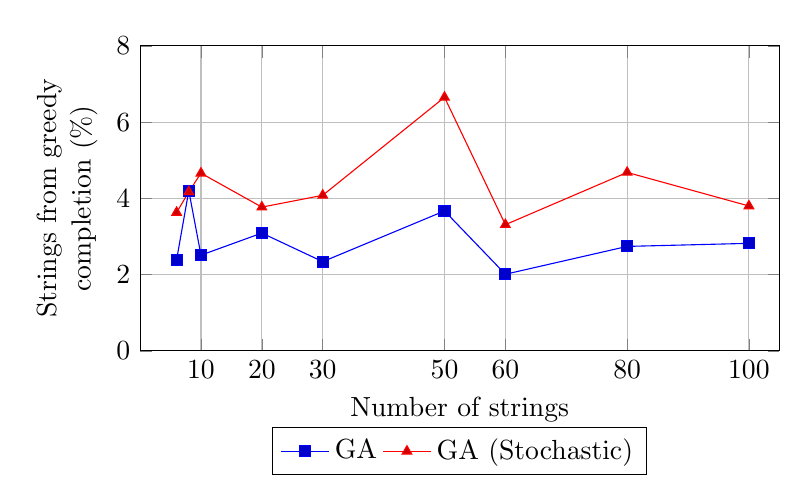
\begin{tikzpicture}
\begin{axis}[
    width=0.8\linewidth,
    height=0.45\linewidth,
    xlabel={Number of strings},
    ylabel={\shortstack{Strings from greedy\\completion (\%)}},
    xmin=0, xmax=105,
    ymin=0, ymax=8,
    xtick={10,20,30,50,60,80,100},
    ytick={0,2,4,6,8},
    ymajorgrids=true,
    xmajorgrids=true,
    legend style={at={(0.5,-0.25)},anchor=north,legend columns=2},
]
\addplot+[mark=square*] coordinates {
  (6,2.39) (8,4.20) (10,2.51) (20,3.09) (30,2.34) (50,3.67) (60,2.01) (80,2.74) (100,2.82)
};
\addlegendentry{GA}

\addplot+[mark=triangle*] coordinates {
  (6,3.63) (8,4.17) (10,4.66) (20,3.77) (30,4.08) (50,6.65) (60,3.31) (80,4.68) (100,3.80)
};
\addlegendentry{GA (Stochastic)}

\end{axis}
\end{tikzpicture}
\caption{Share of string placements produced by the greedy completion step as a function of the number of strings. The complement to $100\%$ can be interpreted as the ``completion rate'' of the crossover operators.}
\label{fig:greedy-share-vs-2Dstrings}
\end{figure}

\section{Conclusion}
\label{sec:conclusion}

This paper has introduced the Two-Dimensional Shortest Superstring Problem (2D-SSP), establishing it as a rich combinatorial optimization problem unifying string sequencing with geometric packing.

\paragraph{Theoretical foundations.}
We established NP-hardness for both objectives and APX-hardness for area via L-reduction from 1D-SSP. The \emph{Bounded-Offset Tree Representation} transforms 2D-SSP from geometric optimization over infinite coordinates into a finite combinatorial problem over spanning trees. The connectivity/compaction theorem (Theorem~\ref{thm:compaction}) proves optimal solutions can be made 4-connected without increasing cost.

\paragraph{Algorithmic innovation.}
Our Memetic Algorithm (T-GA) features locality-preserving crossover that preserves beneficial subtree structures. Crossover dominates solution construction ($>95\%$ of placements), with greedy completion providing lightweight repair. The GA achieves optimality gaps $\le 2.6\%$ on ILP-verifiable instances and outperforms greedy baselines by $6$--$12\%$ on larger instances.

\paragraph{Extensions.}
The theoretical framework extends directly to $d$-dimensional SSP for any $d \ge 1$, with $2d$-adjacency replacing $4$-adjacency; see Appendix~\ref{app:higher-dim}.

\paragraph{Limitations.}
The ILP does not scale beyond $n \le 10$. The gap between existence of optimal trees and the GA's greedy-completion subspace remains theoretically open. Experiments focus on binary alphabets; behavior on higher-entropy instances is unexplored.

\paragraph{Future directions.}
Key open problems include: (1) approximation algorithms generalizing 1D-SSP's $2.5$-approximation; (2) APX-hardness of 2D-SSP$_{\mathrm{bal}}$ in the sequencing regime; (3) scaling exact methods via decomposition or column generation; and (4) extension to non-rectangular patterns.


% ===================== APPENDIX =====================
\appendix

\section{Supplementary Technical Details}
\label{app:supplementary}

This appendix collects extended discussions moved from the main text for space reasons.

\subsection{A planar crossing lemma for the grid}
\label{app:grid-crossing}

The proof of Theorem~\ref{thm:compaction} uses the following standard separation property of the rectangular grid graph.

\begin{lemma}[Grid crossing]
\label{lem:grid-crossing}
Let $W,H\ge 1$ and consider the grid graph with vertex set
\[
V := \{0,\dots,W-1\}\times\{0,\dots,H-1\}
\]
and edges between 4-neighbours (Manhattan distance $1$).
Let $P$ be a vertex-simple path in this graph from the top side (some vertex with $y=H-1$) to the bottom side (some vertex with $y=0$).
Let $Q$ be a vertex-simple path from the left side (some vertex with $x=0$) to the right side (some vertex with $x=W-1$).
Then $P$ and $Q$ share a vertex.
\end{lemma}

\begin{pf}
Embed the grid graph in the plane by placing each vertex $(x,y)$ at its Euclidean position and drawing each edge as a straight-line segment.
The path $P$ together with the boundary of the rectangle forms a closed curve that separates the left side from the right side in the planar embedding (a direct consequence of the Jordan curve theorem; see, e.g., standard texts on planar graphs).
Since $Q$ connects a vertex on the left side to a vertex on the right side using grid edges that do not cross each other, $Q$ must intersect $P$ in the embedding.
Because distinct grid edges intersect only at common endpoints, this intersection must occur at a common vertex of $P$ and $Q$.
\end{pf}

\subsection{APX-Hardness Proof Details}
\label{app:apx-hardness}

Recall that an L-reduction from problem $A$ to problem $B$ requires constants $\alpha, \beta > 0$ such that:
\begin{enumerate}
    \item $\mathrm{OPT}_B \le \alpha \cdot \mathrm{OPT}_A$, and
    \item for any solution to $I_B$ with cost $c_B$, one can construct a solution to $I_A$ with cost $c_A$ satisfying $|c_A - \mathrm{OPT}_A| \le \beta \cdot |c_B - \mathrm{OPT}_B|$.
\end{enumerate}

\emph{Condition (1):} From Theorem~\ref{thm:np-hard}, $\mathrm{OPT}_{2\text{D}} = \mathrm{OPT}_{1\text{D}}$, so $\alpha = 1$.

\emph{Condition (2):} Given any 2D placement with area $A$, the row-concatenation argument in Theorem~\ref{thm:np-hard} produces a 1D superstring of length $\le A$. Thus $c_{1\text{D}} \le c_{2\text{D}}$, which implies $c_{1\text{D}} - \mathrm{OPT}_{1\text{D}} \le c_{2\text{D}} - \mathrm{OPT}_{2\text{D}}$, so $\beta = 1$.

\subsection{Complexity Details: Alphabet Size and Sequencing--Packing Spectrum}
\label{app:complexity-details}

\paragraph{Approximation complexity of 2D-SSP$_{\mathrm{bal}}$.}
The L-reduction does \emph{not} extend to 2D-SSP$_{\mathrm{bal}}$. For height-1 strings, multiple rows can reduce the balanced cost: if $\mathrm{OPT}_{1\text{D}} = 100$ and strings can be arranged in 10 rows of width 10 each, the balanced cost becomes $\max\{10, 10\} = 10 < 100$.

Our NP-hardness proof for 2D-SSP$_{\mathrm{bal}}$ (Theorem~\ref{thm:np-hard-bal}) operates in the \emph{packing regime}: large alphabets force non-overlapping placements, reducing to rectangle packing. However, the \emph{approximation complexity} in the \emph{sequencing regime} (small $|\Sigma|$, frequent overlaps) remains open.

\paragraph{Alphabet size and hardness.}
The case $|\Sigma| = 1$ is trivial: all strings can be stacked at the origin, yielding bounding box equal to the largest string's dimensions. At the opposite extreme ($|\Sigma| \ge n$ with unique symbols), no overlaps are possible and 2D-SSP reduces to rectangle packing.

\paragraph{SSP vs.\ Packing: Opposing objectives.}
In packing problems, the goal is to fit rectangles into a container \emph{without overlap}. In 2D-SSP, overlaps are \emph{encouraged}---they reduce the bounding box. For $|\Sigma| = 1$, 2D-SSP is trivial (maximal overlap permitted) while packing remains NP-hard (no-overlap constraint persists).

\paragraph{Information entropy and the sequencing--packing spectrum.}
The effective difficulty depends on string entropy:
\begin{itemize}
    \item \emph{High entropy (random strings, large $|\Sigma|$):} Probability of symbol-consistent overlap decreases exponentially with overlap size. 2D-SSP degenerates toward a packing problem.
    \item \emph{Low entropy (repetitive strings, small $|\Sigma|$):} Many pairs admit large overlaps. The problem becomes a sequencing problem with combinatorial explosion of valid configurations.
\end{itemize}

Binary alphabets represent the sequencing regime where 2D-SSP is most distinct from pure geometric packing.

\subsection{Edge Density and String Entropy}
\label{app:edge-density}

The bound $O(n^2 wh)$ on $|E(G^{\mathrm{pl}})|$ is a worst-case geometric bound. The set of valid offsets $\mathcal{C}_{ij}$ decomposes as $\mathcal{C}_{ij} = \mathcal{C}_{ij}^{\mathrm{adj}} \cup \mathcal{C}_{ij}^{\mathrm{ovl}}$.

\emph{Adjacency edges} $|\mathcal{C}_{ij}^{\mathrm{adj}}|$: Always present, contributing $O(w_i + w_j + h_i + h_j)$ edges per pair (the perimeter of the contact region).

\emph{Overlap edges} $|\mathcal{C}_{ij}^{\mathrm{ovl}}|$: For symbols drawn uniformly from $\Sigma$, $\Pr[\text{$k$-cell overlap is consistent}] = |\Sigma|^{-k}$. For random strings over large alphabets, $|\mathcal{C}_{ij}^{\mathrm{ovl}}| \approx 0$ and $G^{\mathrm{pl}}$ is sparse.

\emph{Periodic/low-entropy strings}: Many overlaps become symbol-consistent. For $|\Sigma| = 1$, every offset in the contact region is valid, yielding $|\mathcal{C}_{ij}| = O(w_i w_j + h_i h_j)$.

\subsection{Optimized Offset Enumeration}
\label{app:offset-enumeration}

The na\"ive approach enumerates all $O(wh)$ candidate offsets per pair. In the sequencing regime, we can improve performance by iterating offsets in order of \emph{bounding-box increase}.

For two strings $T_i$ ($w_i \times h_i$) and $T_j$ ($w_j \times h_j$), placing $T_j$ at offset $(\Delta x, \Delta y)$ increases the bounding box by a computable amount $\mathrm{inc}(\Delta x, \Delta y)$. We enumerate offsets in non-decreasing order of $\mathrm{inc}$:
\begin{itemize}
    \item $\mathrm{inc} = 0$: Full containment.
    \item $\mathrm{inc} = 1$: Partial overlap leaving 1 row/column exposed.
    \item \ldots up to $\mathrm{inc} = w_j + h_j - 2$ (4-adjacent contact, no overlap).
\end{itemize}

For fixed $\mathrm{inc}$, valid offsets form a predictable geometric ``frame.'' A greedy algorithm can \textbf{stop at the first level containing a symbol-consistent offset}. Worst-case complexity remains $O(wh)$, but average-case improves when overlaps are frequent.

\subsection{Extension to Higher Dimensions}
\label{app:higher-dim}

The theoretical framework extends directly to $d$-dimensional SSP for any $d \ge 1$:

\emph{(i) Geometry:} Objects are hyper-rectangles with dimensions $n_1 \times \cdots \times n_d$. Cost becomes volume $\prod_{k=1}^{d} W_k$ or maximum side $\max_k W_k$. Offsets are vectors $\delta \in \mathbb{Z}^d$. The bounded offset property holds: valid offsets are bounded by the sum of dimensions along each axis.

\emph{(ii) Connectivity lemma:} The sliding argument works in $\mathbb{Z}^d$: disconnected components $A$ and $B$ can be translated along a cardinal axis through empty space until they share a $(d-1)$-dimensional face, without increasing any bounding-box dimension.

\emph{(iii) Graph representation:} 4-connectivity generalizes to $2d$-connectivity (sharing a $(d-1)$-face). The contact graph definition is identical; Corollary~\ref{cor:tree-optimal} holds verbatim with $2d$-adjacency replacing $4$-adjacency.

Applications include 3D voxel assembly, volumetric data compression, and higher-dimensional tensor compression.

\subsection{Existence vs.\ Search Reachability}
\label{app:greedy-gap}

Corollary~\ref{cor:tree-optimal} establishes \emph{existence} of an optimal placement tree, but our GA searches only ``greedily-completable'' trees. A natural question: \emph{can the optimal tree be ``ungreedy''?} That is, might the optimal require a locally suboptimal edge to achieve minimum cost globally?

In principle, yes: the optimal tree might contain an edge $(i,j,\delta)$ dominated by $(i,j,\delta')$ with smaller local cost, yet $\delta$ enables a globally superior arrangement.

Two design choices mitigate this:
\begin{enumerate}
    \item \emph{Stochastic completion} randomly samples among equally-good candidates, exploring alternative attachment points.
    \item \emph{Crossover dominance}: Table~\ref{tab:ga-internals} shows 95--97.5\% of placements are inherited from parents via crossover, not constructed by greedy. The greedy-completion bias affects only a small fraction of solution structure.
\end{enumerate}

Empirically, the GA matches ILP solutions on small instances, suggesting the greedy-completion subspace contains near-optimal solutions for typical inputs.

\subsection{Population Diversity Analysis}
\label{app:population-diversity}

Our greedy completion is \emph{context-sensitive}: placement of each missing string depends on the current canvas state, which varies across offspring.

Table~\ref{tab:ga-internals} confirms:
\begin{itemize}
    \item Crossover dominates: $95$--$97.5\%$ of placements come directly from crossover.
    \item Repair rate $r_{\text{repair}}$ remains bounded at $3$--$13\%$ even as instances scale.
    \item This indicates sustained population diversity rather than convergence to ``super-individuals.''
\end{itemize}

The greedy operator acts as lightweight boundary repair, filling $2$--$5\%$ of solution structure. This is analogous to mutation: essential for feasibility and diversity, but not the primary driver of solution quality.

\section{ILP Formulation Details}
\label{app:ilp-formulation}

This appendix provides the complete mathematical formulation of the mixed-integer linear program used for exact verification of small instances. The main text (Section~\ref{sec:ilp-baseline}) provides an overview; here we present the full technical details.

\subsection{Notation and Grid Setup}

We reuse the notation from Section~\ref{sec:problem}. We have a finite set of 2D strings $\mathcal{T} = \{T_1,\dots,T_n\}$, each represented by a finite set of local cells $C_i \subset \mathbb{Z}^2$ and a symbol function $T_i : C_i \to \Sigma$. For each $i$ we denote the local bounding box of $T_i$ by
\begin{align*}
  x_i^{\min} &= \min_{(u,v)\in C_i} u, &
  x_i^{\max} &= \max_{(u,v)\in C_i} u, \\
  y_i^{\min} &= \min_{(u,v)\in C_i} v, &
  y_i^{\max} &= \max_{(u,v)\in C_i} v,
\end{align*}
and its width and height by
\[
  w_i = x_i^{\max} - x_i^{\min} + 1,
  \qquad
  h_i = y_i^{\max} - y_i^{\min} + 1.
\]

We embed all strings into a common rectangular grid $[0,W_g] \times [0,H_g] \subset \mathbb{Z}^2$. To guarantee that the ILP is a \emph{true exact solver}, the grid must be large enough to accommodate \emph{any} possible optimal arrangement, including those with extreme aspect ratios.

\begin{remark}[Grid bounds and exactness]
\label{rem:grid-bounds}
A na\"ive approach would set $W_g = \sum_i w_i$ and $H_g = \sum_i h_i$ (the maximum possible dimensions if all strings are placed in a line with no overlap). This guarantees global optimality but creates an enormous grid.

A tempting optimization is to use greedy bounds: run a heuristic to obtain dimensions $W_{\text{greedy}} \times H_{\text{greedy}}$, then set $W_g := W_{\text{greedy}}$ and $H_g := H_{\text{greedy}}$. However, this is \emph{not} sound for all objectives:

\begin{itemize}
    \item \emph{For 2D-SSP$_{\mathrm{area}}$:} An optimal solution may have a different aspect ratio than the greedy solution. For example, if greedy yields a $10 \times 10$ placement (area 100), the optimal might be $2 \times 40$ (area 80). If $W_g = H_g = 10$, the ILP would exclude the $2 \times 40$ solution since $40 > 10$.
    
    \item \emph{For 2D-SSP$_{\mathrm{bal}}$:} The greedy bound \emph{is} sound. If greedy achieves $\max\{W_{\text{greedy}}, H_{\text{greedy}}\} = L$, any optimal solution has $\max\{W^*, H^*\} \leq L$, so both dimensions are bounded by $L$.
\end{itemize}

To ensure global exactness for both objectives, we use:
\[
  W_g := \min\Bigl(\sum_i w_i,\; \mathrm{cost}_{\mathrm{area}}^{\text{greedy}}\Bigr), \qquad
  H_g := \min\Bigl(\sum_i h_i,\; \mathrm{cost}_{\mathrm{area}}^{\text{greedy}}\Bigr).
\]
This exploits the fact that if the greedy area is $A_{\text{greedy}}$, any optimal area satisfies $W^* \cdot H^* \leq A_{\text{greedy}}$, so $W^* \leq A_{\text{greedy}}$ (since $H^* \geq 1$). The grid remains bounded by the greedy area rather than the sum of all dimensions, while accommodating all aspect ratios.
\end{remark}

For small verification instances, this grid size is manageable. For larger instances, the ILP becomes intractable regardless of grid bounds.

\subsection{Symmetry Breaking and Candidate Origins}

To eliminate redundant symmetric solutions arising from translation invariance, we apply \emph{symmetry breaking}: we fix the first string $T_1$ at the origin by restricting its set of allowed origins to $\mathcal{O}_1 := \{(0,0)\}$. This constraint removes all translated copies of any given solution from the search space without affecting optimality.

For each string $i \ge 2$ we define a finite set of allowed \emph{origins} $\mathcal{O}_i \subset \mathbb{Z}^2$ such that translating $T_i$ by $o$ keeps all its local cells inside the global grid:
\begin{equation}
  \begin{split}
    \mathcal{O}_i \;:=\; \Bigl\{\, o = (x,y) \in \mathbb{Z}^2 \,\Big|\,
    & (x+u, y+v) \in [0,W_g]\times[0,H_g] \\
    & \text{for all } (u,v)\in C_i \Bigr\}.
  \end{split}
  \label{eq:ilp-origins}
\end{equation}
Recall that $\mathcal{O}_1 = \{(0,0)\}$ by the symmetry-breaking constraint. When $T_i$ is placed at an origin $o = (x,y)$, each local cell $(u,v)\in C_i$ is mapped to global coordinates $(x+u,y+v)$.

\subsection{Conflict Precomputation}

Two candidate placements $(i,o)$ and $(j,o')$ are incompatible if they assign different symbols to the same global coordinate. Formally, we precompute a Boolean conflict indicator
\begin{equation}
  \kappa_{ijoo'} =
  \begin{cases}
    1, & \begin{aligned}[t]
           &\text{if there exist } (u,v)\in C_i,\, (u',v')\in C_j \\
           &\text{with } (x+u,y+v)=(x'+u',y'+v') \\
           &\text{and } T_i(u,v)\neq T_j(u',v'), \\
           &\text{for } o=(x,y),\,o'=(x',y'),
         \end{aligned} \\
    0, & \text{otherwise},
  \end{cases}
  \label{eq:ilp-kappa}
\end{equation}
for all $i<j$, $o\in\mathcal{O}_i$, and $o'\in\mathcal{O}_j$. This preprocessing reduces symbol consistency to simple pairwise constraints in the ILP.

\subsection{Decision Variables}

The model uses the following variables.
\begin{itemize}
  \item For each string $i \in \{1,\dots,n\}$ and each origin $o\in\mathcal{O}_i$:
        \[
          b_{io} \in \{0,1\}
          \quad\text{(1 if $T_i$ is placed at origin $o$, 0 otherwise).}
        \]
  \item Integer coordinates of the global bounding box:
        \[
          X_{\min}, X_{\max}, Y_{\min}, Y_{\max} \in \mathbb{Z},
        \]
        which represent the minimum and maximum global row/column indices among all occupied cells.
  \item The width and height of the bounding box:
        \[
          W, H \in \mathbb{Z}_{\ge 0}.
        \]
  \item A maximum side variable (for the balanced-area objective):
        \[
          L \in \mathbb{Z}_{\ge 0},
        \]
        representing the maximum of width and height.
  \item An area variable (for the area objective):
        \[
          A \in \mathbb{Z}_{\ge 0},
        \]
        used to model or approximate the bounding-box area $W\cdot H$.
\end{itemize}
In the implementation we bound these variables by a constant
\[
  M \;:=\; \max\{W_g, H_g\} + \max_i \max\{w_i,h_i\},
\]
so that $X_{\min},X_{\max},Y_{\min},Y_{\max} \in [-M,M]$ and $W,H,L \in [0,M]$, $A \in [0,M^2]$.

\begin{remark}[Big-$M$ calibration]
\label{rem:big-m}
The choice of $M$ involves a trade-off. If $M$ is too small, valid placements may be incorrectly excluded; if $M$ is excessively large, the LP relaxation becomes weak (the big-$M$ constraints provide little tightening when $b_{io} = 0$), leading to slow branch-and-bound convergence.

Our choice $M = \max\{W_g, H_g\} + \max_i \max\{w_i, h_i\}$ is valid given the grid bounds from Remark~\ref{rem:grid-bounds}: since the grid accommodates all optimal solutions, no coordinate can exceed $\max\{W_g, H_g\}$ plus the maximum string dimension. The bound is instance-adaptive and typically much smaller than a na\"ive bound like $n \cdot \max_i \max\{w_i, h_i\}$, improving LP relaxation quality.
\end{remark}

\subsection{Common Constraints}

Both objective variants share the following groups of constraints.

\medskip
\noindent
\emph{(i) Exactly one origin per string.}
Each 2D string must be placed at exactly one origin:
\begin{equation}
  \sum_{o\in\mathcal{O}_i} b_{io} \;=\; 1
  \qquad \forall i \in \{1,\dots,n\}.
  \label{eq:ilp-one-origin}
\end{equation}

\medskip
\noindent
\emph{(ii) No symbol conflicts.}
If two candidate placements $(i,o)$ and $(j,o')$ conflict, they cannot be chosen simultaneously:
\begin{equation}
  b_{io} + b_{jo'} \;\le\; 1
  \quad
  \forall\, i<j,\ \forall\, o\in\mathcal{O}_i,\ \forall\, o'\in\mathcal{O}_j
  \text{ with } \kappa_{ijoo'} = 1.
  \label{eq:ilp-conflict}
\end{equation}

\medskip
\noindent
\emph{(iii) Bounding box must contain all placed strings.}
Let $o=(x,y)\in\mathcal{O}_i$ be a candidate origin for $T_i$. If $b_{io}=1$, then the global footprint of $T_i$ is
\[
  [x + x_i^{\min},\, x + x_i^{\max}]
  \times
  [y + y_i^{\min},\, y + y_i^{\max}],
\]
and this rectangle must lie inside $[X_{\min},X_{\max}]\times[Y_{\min},Y_{\max}]$. We encode these implications with big-$M$ constraints:
\begin{align}
  X_{\min} &\;\le\; x + x_i^{\min} + M(1-b_{io}),
  \label{eq:ilp-Xmin} \\
  X_{\max} &\;\ge\; x + x_i^{\max} - M(1-b_{io}),
  \label{eq:ilp-Xmax} \\
  Y_{\min} &\;\le\; y + y_i^{\min} + M(1-b_{io}),
  \label{eq:ilp-Ymin} \\
  Y_{\max} &\;\ge\; y + y_i^{\max} - M(1-b_{io}),
  \label{eq:ilp-Ymax}
\end{align}
for all $i$ and all $o=(x,y)\in\mathcal{O}_i$. When $b_{io}=1$ these reduce to the desired inequalities $X_{\min}\le x+x_i^{\min}$, $X_{\max}\ge x+x_i^{\max}$, etc., and when $b_{io}=0$ they are relaxed by the big-$M$ terms.

\medskip
\noindent
\emph{(iv) Definition of width and height.}
The bounding box dimensions are defined by
\begin{equation}
  W = X_{\max} - X_{\min} + 1,
  \qquad
  H = Y_{\max} - Y_{\min} + 1.
  \label{eq:ilp-WH}
\end{equation}
In addition, $W$ and $H$ must be at least as large as the widest and tallest individual 2D string:
\begin{equation}
  W \;\ge\; \max_i w_i,
  \qquad
  H \;\ge\; \max_i h_i.
  \label{eq:ilp-WH-lb}
\end{equation}

\subsection{Balanced-Area Objective}

The balanced-area variant minimises the maximum side length $\max\{W,H\}$. We link $L$ to $W$ and $H$ via
\begin{equation}
  L \;\ge\; W,
  \qquad
  L \;\ge\; H.
  \label{eq:ilp-bal-L}
\end{equation}
At optimality, $L = \max\{W,H\}$.

The \emph{balanced-area} ILP is
\begin{align}
  \min \quad & L
  \label{eq:ilp-bal-obj} \\
  \text{s.t.} \quad
  &\eqref{eq:ilp-one-origin} - \eqref{eq:ilp-WH-lb},\ \eqref{eq:ilp-bal-L}, \nonumber \\
  &b_{io} \in \{0,1\}\ \forall i,o,\quad
   X_{\min},X_{\max},Y_{\min},Y_{\max},W,H,L \in \mathbb{Z}. \nonumber
\end{align}

\subsection{Area Objective}

The area-based variant uses the product $W\cdot H$ as its cost. Conceptually we want
\begin{equation}
  A = W \cdot H.
  \label{eq:ilp-area-ideal}
\end{equation}

\begin{remark}[Linearization of the bilinear term]
\label{rem:linearization}
The product $W \cdot H$ makes the area objective inherently \emph{non-convex}. A direct formulation would yield a Mixed-Integer \emph{Nonlinear} Program (MINLP), which is significantly harder to solve than a Mixed-Integer \emph{Linear} Program (MILP).

We linearize this bilinear term using the \emph{McCormick envelope}, the tightest convex relaxation of the product over a box. This is a standard technique in global optimization~\citep{mccormick1976computability}. The McCormick envelope provides the \emph{convex hull} of points $(W, H, W \cdot H)$ when $W$ and $H$ are continuous, but for integer variables, it is only a relaxation: intermediate points satisfying the envelope constraints may not correspond to integer solutions with $A = W \cdot H$.

For our small verification instances, this relaxation is tight in practice: the branch-and-bound solver finds integer solutions where the McCormick constraints are binding. Alternative approaches for tighter formulations include:
\begin{itemize}
    \item \emph{Logarithmic discretization:} Introduce binary variables for each bit of $W$ and $H$, yielding $O(\log W_{\max} \cdot \log H_{\max})$ auxiliary variables and an exact linearization.
    \item \emph{SOS2 piecewise-linear approximation:} Approximate $W \cdot H$ using special ordered sets of type 2, trading exactness for tighter LP relaxations.
    \item \emph{Surrogate minimization:} Since we minimize area, we could minimize $(W + H)$ as a surrogate (perimeter), which is linear. However, this changes the objective and may yield suboptimal area solutions.
\end{itemize}
We chose McCormick for simplicity, as it sufficed for our small test cases. For larger instances requiring tighter relaxations, logarithmic discretization would be preferred.

In contrast, the balanced objective $\max\{W, H\}$ is trivially linearized via auxiliary variable $L \geq W$, $L \geq H$, no relaxation is needed.
\end{remark}

To remain within a MILP framework we linearize this product over a known box $W \in [W_{\min},W_{\max}]$, $H \in [H_{\min},H_{\max}]$. We take
\[
  W_{\min} := \max_i w_i,\quad
  H_{\min} := \max_i h_i,\quad
  W_{\max},H_{\max} \le M,
\]
and impose the standard McCormick envelope
\begin{align}
  A &\;\ge\; W_{\min} H + H_{\min} W - W_{\min} H_{\min},
  \label{eq:ilp-mcc-1} \\
  A &\;\ge\; W_{\max} H + H_{\max} W - W_{\max} H_{\max},
  \label{eq:ilp-mcc-2} \\
  A &\;\le\; W_{\min} H + H_{\max} W - W_{\min} H_{\max},
  \label{eq:ilp-mcc-3} \\
  A &\;\le\; W_{\max} H + H_{\min} W - W_{\max} H_{\min}.
  \label{eq:ilp-mcc-4}
\end{align}
These constraints define the convex hull of all triples $(W,H,A)$ with $A=W\cdot H$ and $(W,H)$ in the given box. On small instances one can further tighten this relaxation by introducing a discrete piecewise-linear approximation of $W\cdot H$, but the simple McCormick envelope above already proved sufficient for our experiments.

The \emph{bounding area} ILP is
\begin{align}
  \min \quad & A
  \label{eq:ilp-area-obj} \\
  \text{s.t.} \quad
  &\eqref{eq:ilp-one-origin} - \eqref{eq:ilp-WH-lb},\ \eqref{eq:ilp-mcc-1} - \eqref{eq:ilp-mcc-4}, \nonumber \\
  &b_{io} \in \{0,1\}\ \forall i,o,\quad
   X_{\min},X_{\max},Y_{\min},Y_{\max},W,H,A \in \mathbb{Z}. \nonumber
\end{align}
The objective value $A^\star$ coincides with the area of the minimal axis-aligned bounding rectangle $B(p)$ enclosing all occupied cells in the induced placement $p$.

\medskip
This formulation is conceptually straightforward: each $b_{io}$ encodes a specific choice of origin for string $T_i$; the conflict constraints \eqref{eq:ilp-conflict} enforce symbol consistency; the big-$M$ constraints \eqref{eq:ilp-Xmin}--\eqref{eq:ilp-Ymax} define a global bounding box that contains all chosen placements; and depending on the variant, either \eqref{eq:ilp-bal-L} or \eqref{eq:ilp-mcc-1}--\eqref{eq:ilp-mcc-4} expresses the chosen cost. The greedy-based grid bounds and symmetry breaking significantly reduce the search space, but the number of variables and conflict constraints still grows quickly with the number of strings.


% ===================== BACK MATTER =====================

%% Bibliography - Harvard style for Computers & Operations Research
\bibliographystyle{elsarticle-harv}
\bibliography{references}

\end{document}
